\pdfoutput=1
\synctex=1
\documentclass[english,a4paper]{lmcs}

\usepackage{amsmath,amsthm,amssymb}
\usepackage{enumitem}
\usepackage{tikz,tikz-cd}
\usepackage{microtype}
\usepackage[mathscr]{euscript}
\usepackage{mathtools}
\usepackage{thmtools,thm-restate}

% fundamental group notation uses this
\usepackage{upgreek}

% only for writing. Remove in the final version.
\usepackage{todonotes}

% load hyperref last
\usepackage{hyperref}

% except for cleveref
\usepackage[capitalize]{cleveref}

\pdfadjustspacing=1
\brokenpenalty=10000 %%% No hyphenation across page breaks
\mathtoolsset{mathic}

%\input macros%
\input macros2%

\def\githubpath{\tt\small}

\hypersetup{
    colorlinks,
    linkcolor={red!50!black},
    citecolor={blue!50!black},
    urlcolor={blue!80!black}
}

\setlist[enumerate]{label=(\roman*)}

\newif\ifarxiv
\arxivtrue
\ifarxiv
  \renewcommand{\datename}{}
  \renewcommand{\headertextsf}[1]{}
\fi

\begin{document}

\title{On symmetries of spheres in univalent foundations}

\author{Pierre Cagne}
\address{Universitetet i Bergen}

\author{Ulrik Buchholtz}
\address{Technische Universit\"at Darmstadt}

\author{Nicolai Kraus}
\address{University of Nottingham}

\author{Marc Bezem}
\address{Universitetet i Bergen}

\date{\normalsize Last updated on \today}%

\begin{abstract}
  In this paper, we investigate the symmetries of the spheres in
  univalent foundations.  The case of the circle has a slick answer:
  the symmetries of the circle form two copies of the circle. For
  higher-dimensional spheres, there are again two connected
  components, corresponding to maps of degree plus or minus one, but
  the components are no longer spheres, as their lowest degree
  homotopy groups have order two.
\end{abstract}

\maketitle

\section{Introduction}

In this paper, we are interested in the description of the type
$\Sn n = \Sn n$ ($n\geq 1$) where $\Sn n$ is the $n$-dimensional
sphere, as defined in the HoTT-book (cf.~\cite{HoTT}).

To be fully precise and to fix notations, we work inside an
intuitionistic Martin-Löf's type theory with $\Sigma$-, $\Pi$- and
$\Id$-types and with a cumulative hierarchy of universes,
simply written $\UU$, for which Voevodsky's univalence axiom hold. The
transport along $p$ in a type family $T:A\to \UU$ is denoted
$\trp [T] p$, and $\pathover u T p v$ denotes $\trp [T] p {(u)} = v$.
For any dependent function $f\from\prod_{x\from A}T(x)$,
the function
\begin{displaymath}
  \ap f:\prod_{x,y\from A}\prod_{p\from x=y} \pathover {f(x)} T p
  {f(y)}
\end{displaymath}
denotes the dependent application of $f$. We usually leave out the two
first arguments of $\ap f$ as they are inferable, and we write simply
$\ap f (p)$ for a path $p:x=y$. As in \cite{HoTT}, we call a type $A$
a \emph{proposition} if the type $\prod_{x,y\from A} x=y$ contains an
element.

We deviate from \cite{HoTT} in denoting path composition:
if $p:x=y$ and $q:y=z$ are paths, then we denote their
composition by $qp$, or by $q\cdot p$.

We postulate a type $\NN$ of natural numbers with its inductive property
(cf.~\cite[Chapter 1.9]{HoTT}), from which is crafted a type $\ZZ$ of integers
as in \cite[\githubpath core/lib/types/Int.agda]{hott-agda}. The crucial
property of $\ZZ$ (proved in previously cited file), is that it has decidable
equality. We allow also several higher inductive types that are defined in
\cite{HoTT}: propositional and set truncations, suspension, and the circle.
Considering their importance in this paper, we recall them in full:
\begin{enumerate}
\item the \emph{propositional truncation} of a type $A$ is a type $\Trunc A$
  defined by
  \begin{itemize}
  \item a map $\trunc \blank \from A \to \Trunc A$, and
  \item a dependent function
    $\istrunc {-1} \from \prod_{x,y\from \Trunc A} x=y$
  \end{itemize}
  with the following induction rule:
  \begin{quote}
    given a type family $T\from \Trunc A \to \UU$ such that
    $T(x)$ is a proposition for each $x\from \Trunc A$, every
    dependent function
    \begin{displaymath}
      s\from \prod_{a\from A}T(\trunc a)
    \end{displaymath}
    defines a dependent function
    \begin{displaymath}
      \ind(s)\from\prod_{x\from \Trunc A} T(x)
    \end{displaymath}
    such that $\ind(s)(\trunc a) \jdeq s(a)$ for all $a\from A$.
  \end{quote}
\item the \emph{set truncation} of a type $A$ is a type $\setTrunc A$
  defined by
  \begin{itemize}
  \item a map $\settrunc \blank \from A \to \setTrunc A$, and
  \item a dependent function
    $\istrunc {0} \from \prod_{x,y\from \setTrunc A}\prod_{p,q: x=y} p = q$
  \end{itemize}
  with the following induction rule:
  \begin{quote}
    given a type family $T\from \setTrunc A \to \UU$ such that
    $T(x)$ is a set for each $x\from \setTrunc A$, every
    dependent function
    \begin{displaymath}
      s\from \prod_{a\from A}T(\settrunc a)
    \end{displaymath}
    defines a dependent function
    \begin{displaymath}
      \ind(s)\from\prod_{x\from \setTrunc A} T(x)
    \end{displaymath}
    such that $\ind(s)(\settrunc a) \jdeq s(a)$ for all $a\from A$.
  \end{quote}

\item the \emph{suspension} of a type $A$ is a type $\susp A$ defined
  by
  \begin{itemize}
  \item two elements $\north,\south\from \susp A$, and
  \item a  map $\mrd \from A \to (\north=\south)$
  \end{itemize}
  with the following induction rule:
  \begin{quote}
    given a type family $T\from \susp A \to \UU$, every dependent
    triple of elements
    \begin{displaymath}
      n\from T(\north), \quad s\from T(\south),\quad
      m\from \prod_{a\from A}\pathover n T {\mrd a} s
    \end{displaymath}
    defines a dependent function
    \begin{displaymath}
      \ind(n,s,m)\from\prod_{x\from \susp A} T(x)
    \end{displaymath}
    such that
    \begin{gather*}
      \ind(n,s,m)(\north) \jdeq n,\quad
      \ind(n,s,m)(\south) \jdeq s,\\
      \ap{\ind(n,s,m)}(\mrd a) = m(a)\ \text{for all $a\from A.$}
    \end{gather*}
  \end{quote}
\item the \emph{circle} $\Sc$ is a type defined by
  \begin{itemize}
  \item an element $\base \from \Sc$, and
  \item a path $\Sloop: \base = \base$
  \end{itemize}
  with the following induction rule:
  \begin{quote}
    given a type family $T\from \Sc \to \UU$, every dependent pair of
    elements
    \begin{displaymath}
      b\from T(\base), \quad \ell\from \pathover b T \Sloop b
    \end{displaymath}
    defines a dependent function
    \begin{displaymath}
      \ind(b,\ell)\from\prod_{x\from \Sc} T(x)
    \end{displaymath}
    such that
    \begin{displaymath}
      \ind(b,\ell)(\base) \jdeq b,\quad \ap{\ind(b,\ell)}(\Sloop) = \ell \,.
    \end{displaymath}
  \end{quote}
\end{enumerate}
The spheres $\Sn n$ are then defined by induction on $n:\NN$ by
$\Sn n \defequi \susp(\Sn{n-1})$ for all $n\geq 2$.
We also set $\Sn{-1} \defequi\emptytype$ and $\Sn{0}\defequi\bn 2$.
Then we have $\Sn n = \susp(\Sn{n-1})$ for all $n\ge0$.

\paragraph{Plan of the paper.}%
In \cref{sec:circle-case}, we show carefully that the type $\Sc = \Sc$
is equivalent to $\Sc + \Sc$. Maybe surprising at first, this result
is quite straightforward once we unravel the details.

In \cref{sec:sphere}, we deal with the case $n=2$. Because the
equivalence of the case $n=1$ relies heavily on $\Omega(\Sc)\weq \ZZ$
being an abelian group, we can not expect to generalize the proof for
$n=2$. However, a careful analysis of Brunerie's proof of
$\pi_2(\Sp) \weq \ZZ$ allows us to prove that the type $\Sp=\Sp$ has
exactly two connected components, equivalent to one another.
Determining a type with a simple description that is
equivalent to these components is a challenge in itself, still open,
to the authors' knowledge.

In \cref{sec:higher-sphere}, we propagate the result by induction on
$n\geq 2$: the type $\Sn n = \Sn n$ has exactly two connected
components, equivalent to one another. Each induction step relies on
Freudenthal's suspension theorem.

In \cref{sec:structure-components}, we then show that the fundamental group of each component is $\ZZ/2\ZZ$ for $n\ge2$.
We partly develop an EHP long exact sequence to deal with the case $n=2$.

\section{Symmetries of the circle}
\label{sec:circle-case}%

In this section, we will prove the following result.
\begin{thm}
  \label{thm:symmetries-of-S1}
  There is an equivalence
  \begin{equation}
    \label{eq:symm-cricle}%
    (\Sc = \Sc) \weq \Sc+\Sc.
  \end{equation}
\end{thm}
We will treat univalence as transparent, so that equivalences
$f:\Sc\weq \Sc$ will be treated as elements of $\Sc=\Sc$ without any
warning. In particular, we shall write as if
``$\refl \Sc \jdeq \id_\Sc$''.

To provide an equivalence of type \cref{eq:symm-cricle}, we proceed
in several steps:
\begin{itemize}
\item first, we will describe two elements of $\Sc=\Sc$;
\item next, we will prove that these two elements are not equal (and
hence in different connected components);
\item then, we will prove that every equivalence in $\Sc=\Sc$ is
  merely equal to one of these two elements;
\item finally, we will conclude by exhibiting an equivalence between
  $\Sc$ and the connected component of each of these two elements.
\end{itemize}

The first element is simply the identity equivalence $\id_\Sc$. The
second element is the function
$-\id_\Sc \defequi \ind(\base,\inv{\Sloop})$ defined by
$\Sc$-induction in the constant type family at $\Sc$. In other words,
$-\id_\Sc$ is the (propositionally) unique function $\Sc \to \Sc$ such
that:
\begin{displaymath}
  -\id_\Sc(\base) \jdeq \base%
  \quad\text{and}\quad%
  \ap{-\id_\Sc}(\Sloop) = \inv{\Sloop}.
\end{displaymath}

Let us note that $-\id_\Sc$ is an equivalence. It is indeed its own inverse, as
it is shown in the following. In order to construct a proof of $-\id_\Sc \circ
-\id_\Sc = \id_\Sc$, we use function extensionality and $\Sc$-induction.
$\refl\base$ is an element of $-\id_\Sc\circ -\id_\Sc (\base) = \base$, and
we only need to provide an element of $\pathover {\refl\base} T \Sloop
{\refl\base}$ where $T$ is the type family $x \mapsto -\id_\Sc \circ -\id_\Sc (x)
= x$. The transport in the type family $T$ over $\Sloop$ is given by
\begin{displaymath}
  p \mapsto \Sloop \cdot p \cdot \inv{[-\id_\Sc \circ -\id_\Sc](\Sloop)}.
\end{displaymath}
By definition of $-\id_\Sc$, the formula can be rewritten as $\Sloop \cdot p
\cdot \inv \Sloop$.  Hence $\trp[T] \Sloop (\refl\base) = \refl\base$ by simple
path algebra, as wanted.

\begin{lem}
  \label{lemma:S1-id-neq-minusid}%
  The proposition $\id_\Sc \neq -\id_\Sc$ holds.
\end{lem}
\begin{proof}
  Suppose a path $p\from\id_\Sc = -\id_\Sc$ and derive a
  contradiction. Through function extensionality, and because
  $\id_\Sc(\base) \jdeq \base \jdeq -\id_\Sc(\base)$, one gets a path
  $p(\base) \from \base = \base$, and a $2$-path
  $\ap p (\Sloop) \from \pathover {p(\base)} T \Sloop {p(\base)}$ where
  $T(x)\defequi (\id_\Sc(x) = -\id_\Sc(x))$ for all $x:\Sc$. One can
  easily find by induction on $q\from x=y$ a 2-path of type
  \begin{displaymath}
    \trp [T] q (\blank) = \ap{-\id_\Sc}(q) \blank \inv{\ap{\id_\Sc}(q)}.
  \end{displaymath}
  By composition, $\ap p (\Sloop)$ provides a 2-path of type
  $\inv\Sloop p(\base) \inv\Sloop = p(\base)$. Now recall that
  the function
  \begin{equation}
    \label{eq:loopspace-circle-Z}%
    \ZZ\to(\base=\base),\quad k \mapsto \Sloop^k
  \end{equation}
  is an equivalence. In particular, it shows that path-composition in
  $\base=\base$ is commutative, and $\ap p (\Sloop)$ together with
  path algebra provide then a path of type $\Sloop = \inv\Sloop$. This
  is a contradiction, as it would yield a path of type $1=-1$ in $\ZZ$
  through the equivalence of \cref{eq:loopspace-circle-Z}.
\end{proof}
\cref{lemma:S1-id-neq-minusid} proves that $\id_\Sc$ and $-\id_\Sc$
lie in different connected components of $\Sc=\Sc$. We will now prove
that there are no more connected components in $\Sc=\Sc$. We will need
the following consequence of \cref{lemma:S1-id-neq-minusid}.
\begin{cor}%
  \label{cor:S1-eq-either-isaprop}%
  For every equivalence $\varphi\from \Sc=\Sc$, the following type is
  a proposition:
  \begin{equation}
    \label{eq:S1-def-target-eq}%
    P(\varphi) \defequi \Trunc{\varphi = \id_\Sc} + \Trunc{\varphi = -\id_\Sc}.
  \end{equation}
\end{cor}
\begin{proof}
  The type $P(\varphi)$ is the disjoint sum of two propositions. In
  order to be a proposition, it is enough (and in fact necessary) for
  the two summands to not overlap. More precisely, we need to show
  that the premise
  $\Trunc{\varphi = \id_\Sc}\times\Trunc{\varphi = -\id_\Sc}$ leads to
  absurdity. Absurdity is a proposition, so we can as well suppose the
  premise ${(\varphi = \id_\Sc)}\times{(\varphi = -\id_\Sc)}$. By
  composition of paths, it gives a path of type $\id_\Sc = -\id_\Sc$
  and \cref{lemma:S1-id-neq-minusid} allows us to derive a
  contradiction.
\end{proof}

\begin{prop}
  \label{prop:S1-eq-either}%
  For every equivalence $\varphi\from\Sc=\Sc$, the proposition
  $P(\varphi)$ of \cref{eq:S1-def-target-eq} holds.
\end{prop}
\begin{proof}
  Let $\varphi$ be a symmetry of the circle, and let $\psi$ denote a
  quasi-inverse of $\varphi$. The type $\Sc$ being connected, one
  has $\Trunc{\varphi(\base) = \base}$ and
  $\Trunc{\psi(\base) = \base}$. Because the goal $P(\varphi)$ is
  propositional, one can instead suppose actual paths
  $\varphi_0\from \varphi(\base) = \base$ and
  $\psi_0\from \psi(\base) = \base$. In other words, we can suppose that
  $\varphi$ and its quasi-inverse $\psi$ are pointed maps. Denote
  $\pi$ for a path of type $\varphi\psi = \id_\Sc$. Then one can craft a
  path $(\pi,)$ of type
  $(\varphi,\varphi_0) \circ (\psi,\psi_0) =
  (\id_\Sc, \varphi_0 \cdot \ap \varphi (\psi_0) \cdot \inv {\pi_{\base}})$. Now, consider the
  induced applications
  \begin{displaymath}
    \loopspace{} (\varphi,\varphi_0) \from \loopspace{} \Sc \to \loopspace{} \Sc
    \quad\text{and}\quad
    \loopspace{} (\psi,\psi_0) \from \loopspace{} \Sc \to \loopspace{} \Sc.
  \end{displaymath}
  The elements $\loopspace{} (\varphi,\varphi_0) (\Sloop)$ and
  $\loopspace{} (\psi,\psi_0) (\Sloop)$ of $(\base=\base)$ must be a
  power of $\Sloop$ by the equivalence
  of~\cref{eq:loopspace-circle-Z}. We denote them $\Sloop^k$ and
  $\Sloop^\ell$ respectively. Then the following chain of propositions
  holds:
  \begin{align*}
    \Sloop^{k\ell} &= (\Sloop^k)^\ell\\
    &= \loopspace{} (\varphi,\varphi_0) \left(
      \loopspace{} (\psi,\psi_0) (\Sloop)
    \right)\\
    &= \loopspace{} (\id_\Sc,
    \varphi_0 \cdot \ap \varphi (\psi_0) \cdot \inv {\pi_{\base}} (\Sloop))
    \\
    &=
    \left( \varphi_0 \cdot \ap \varphi (\psi_0) \cdot \inv {\pi_{\base}} \right)
    \cdot \Sloop \cdot
    \inv {\left( \varphi_0 \cdot \ap \varphi (\psi_0) \cdot \inv {\pi_{\base}} \right)}
    \\
    &= \Sloop
  \end{align*}
  where the last equality exploits commutativity of path composition
  in the loop space $(\base = \base)$. Through the equivalence
  of~\cref{eq:loopspace-circle-Z}, we get that $k\ell=1$ in $\ZZ$,
  and by the decidability of equality in $\ZZ$ we get an element of $(k=1)+(k=-1)$.
  From $k=1$, and because
  $\loopspace{} (\varphi,\varphi_0) \jdeq \varphi_0
  \ap\varphi(\Sloop) \inv {\varphi_0}$, one gets an element
  \begin{displaymath}
    b\from \varphi_0 \ap\varphi(\Sloop) \inv {\varphi_0} = \Sloop.
  \end{displaymath}
  One can then construct an element $\kappa\from \varphi = \id_\Sc$ by
  $\Sc$-induction by taking $\kappa(\base)$ to be
  $\varphi_0 \from (\varphi(\base) = \base)$ and $\ap \kappa(\Sloop)$
  the element $b$ just defined, transported back over the equivalence
  \begin{displaymath}
    (\pathover {\varphi_0} {\varphi(\blank) = \id_\Sc(\blank)} \Sloop {\varphi_0}) \weq
    ( \Sloop \varphi_0 \inv {\ap\varphi(\Sloop)} = \varphi_0)
    \weq (\varphi_0 \ap\varphi(\Sloop) \inv {\varphi_0} = \Sloop)
  \end{displaymath}
  By taking $\trunc{\kappa}$, we get an element of
  $\Trunc{\varphi = \id_\Sc}$. Similarly, from $k=-1$, one gets an
  element of $\Trunc{\varphi = -\id_\Sc}$. So in both cases, one gets
  an element of $P(\varphi)$.
\end{proof}

For any type $A$, and an element $a\from A$, let us write $\conncomp A a$
for the connected component of $a$ in $A$. In other words,
\begin{displaymath}
  \conncomp A a \defequi \sum_{x\from A}\Trunc{a=x}.
\end{displaymath}
\cref{lemma:S1-id-neq-minusid} and \cref{prop:S1-eq-either} put
together show that the type $\Sc=\Sc$ has two connected components,
one is the connected component of $\id_\Sc$ and the other is the
connected component of $-\id_\Sc$. In summary, we have shown that
there is an element of the type:
\begin{displaymath}
  (\Sc=\Sc) \weq \conncomp{(\Sc=\Sc)}{\id_\Sc} + \conncomp{(\Sc=\Sc)}{-\id_\Sc}.
\end{displaymath}

In order to prove our goal (cf.~\cref{eq:symm-cricle}), it remains to
exhibit equivalences from $\Sc$ to both
$\conncomp{(\Sc=\Sc)}{\id_\Sc}$ and
$\conncomp{(\Sc=\Sc)}{-\id_\Sc}$. First note that because $\Sc=\Sc$ is
a subtype of $\Sc\to\Sc$, the connected component of any equivalence
$\varphi$ in $\Sc=\Sc$ is equivalent to the connected component of
$\varphi$ seen as a function in $\Sc \to \Sc$. In particular,
\begin{displaymath}
  \conncomp{\left(\Sc=\Sc\right)}{\id_\Sc} \weq \conncomp{\left(\Sc\to\Sc\right)}{\id_\Sc}
  \quad\text{and}\quad
  \conncomp{\left(\Sc=\Sc\right)}{-\id_\Sc} \weq \conncomp{\left(\Sc\to\Sc\right)}{-\id_\Sc}.
\end{displaymath}
Recall that there is an element
\begin{equation}
  \label{eq:S1-loopspace-Z-at-each-x}%
  f\from \prod_{x:\Sc} (\base=\base) \weq (x=x)
\end{equation}
defined by
$\Sc$-induction as the dependent function such that
$f(\base) \jdeq \id_{\base=\base}$ and such that the element
$\ap f (\Sloop) \from (\Sloop\blank\inv\Sloop = \id_{\base=\base})$ is
the reflexivity path of $\id_{\base=\base}$ transported using
commutativity in $\base=\base$ and path algebra.
Because $(\base=\base)$ is equivalent
to $\ZZ$ (cf.~\cref{eq:loopspace-circle-Z}), it gives an equivalence
$\varepsilon_x\from (x=x) \weq \ZZ$ for any $x\from\Sc$. We can now
exhibit an equivalence:
\begin{displaymath}
  \begin{tikzcd}
    \left(\Sc \to \Sc\right) \rar["\weq"] & (\sum_{x\from\Sc}x=x)
    \rar["\weq"] & \Sc \times \ZZ
    \\
    \varphi \rar[mapsto] & (\varphi(\base),\ap \varphi (\Sloop))
    \rar[mapsto] & \left(%
      \varphi(\base), \varepsilon_{\varphi(\base)}(\ap\varphi(\Sloop))%
    \right)%
\end{tikzcd}
\end{displaymath}
In particular, one can verify that $\id_\Sc$ is mapped to $(\base,1)$
and $-\id_\Sc$ is mapped to $(\base,-1)$ through this
equivalence. Because $\ZZ$ is a set and $\Sc$ is connected, the
connected components of $\Sc\times\ZZ$ are easy to understand: for
every $x:\Sc$ and $k:\ZZ$, the connected component of $(x,k)$ is
equivalent to the type of all pairs $(x',k)$ for
$x'\from\Sc$. In particular, every connected component of
$\Sc\times\ZZ$ is equivalent to $\Sc$. In particular, one gets
equivalences:
\begin{displaymath}
  \conncomp{\left(\Sc \to \Sc\right)}{\id_\Sc} \weq \Sc
  \quad\text{and}\quad
  \conncomp{\left(\Sc \to \Sc\right)}{-\id_\Sc} \weq \Sc
\end{displaymath}

Finally, one can compose all the equivalences that we exhibited:
\begin{align*}
  (\Sc=\Sc)
  & \weq \conncomp{\left(\Sc = \Sc\right)}{\id_\Sc}
    + \conncomp{\left(\Sc = \Sc\right)}{-\id_\Sc}
  \\
  & \weq \conncomp{\left(\Sc \to \Sc\right)}{\id_\Sc}
    + \conncomp{\left(\Sc \to \Sc\right)}{-\id_\Sc}
  \\
  & \weq \Sc + \Sc.
\end{align*}

\section{Symmetries of the \texorpdfstring{$2$}{2}-sphere}
\label{sec:sphere}

In this section, we will prove that the canonical inclusion:
\begin{equation}
  \label{eq:goal-section-sphere}
  \conncomp{\left(\Sp = \Sp\right)}{\id_\Sp} +
  \conncomp{\left(\Sp = \Sp\right)}{-\id_\Sp}
  \to
  \left(\Sp = \Sp\right)
\end{equation}
is an equivalence. The equivalence $-\id_\Sp \from \Sp \to \Sp$ is
defined by $\Sp$-induction as the function such that
$-\id_\Sp(\north) \jdeq \south$, and $-\id_\Sp(\south) \jdeq \north$ and
$\ap{-\id_\Sp}(\mrd(x)) = \inv{(\mrd(x))}$ for all $x\from\Sc$.

\begin{lem}
  The function $-\id_\Sp$ is an equivalence.
  \label{lem:minus-id-equivalence}
\end{lem}
\begin{proof}
  We are to produce an element of the type $\prod_{x:\Sp}T(x)$,
  where $T$ is the type family defined by
  $T(x)\defequi (x= (-\id_\Sp \circ -\id_\Sp)(x))$.
  Let us use $\Sp$-induction for this purpose.
  By definition of $-\id_\Sp$,
  $T(\north) \jdeq (\north=\north)$
  and $T(\south) \jdeq (\south=\south)$.
  Hence one can take $\refl \north:T(\north)$
  and $\refl \south:T(\south)$.
  To complete $\Sp$-induction, one should now provide an element
  of type $\prod_{y:\Sc} \pathover{\refl \north} T {\mrd y} {\refl \south}$.
  However,
  transporting over a meridian in the family $T$ is conjugation by the
  meridian: indeed, the transport over any path $p:x=x'$ in $T$ is given by
  $q\mapsto \ap{-\id_\Sp \circ -\id_\Sp}(p) \cdot q \cdot \inv p$, and
  \begin{align*}
    \ap{-\id_\Sp \circ -\id_\Sp} (\mrd(y))
     &= \ap{-\id_\Sp}(\inv {\mrd(y)})
    \\ &= \inv {\left( \ap{-\id_\Sp}(\mrd(y)) \right)}
    \\ &= \inv { \left( \inv{\mrd(y)} \right) }
    \\ &= \mrd(y).
  \end{align*}
  Hence $\pathover{\refl \north} T {\mrd(y)} {\refl \south}$
  is equivalent to
  $\mrd(y)\refl \north \inv {\mrd(y)} = \refl\south$, which is indeed inhabited for any
  $y:\Sc$ by simple path algebra.
\end{proof}

We will follow more or less the same road map as
in~\cref{sec:circle-case}:
\begin{itemize}
\item First, we will prove that $\id_\Sp$ and $-\id_\Sp$ are not in
  the same connected component;
\item then, we will prove that every equivalence in $\Sp=\Sp$ is
  either in the connected component of $\id_\Sp$ or in the connected
  component of $-\id_\Sp$;
\item finally, we will prove that the connected components of $\id_\Sp$
  and $-\id_\Sp$ are equivalent to each other.
\end{itemize}
Notice that the last step is less ambitious than in the case of $\Sc$,
where the two connected components were proven equivalent to each
other but also each equivalent to $\Sc$ itself. Although we do not
have any counter-argument for it, we do not expect that the connected
components of $\id_\Sp$ and $-\id_\Sp$ are each equivalent to $\Sp$
itself. Indeed, the proof in the case of $\Sc$ relies heavily on two
facts: $\Sc$ is $1$-truncated and $\Sc$ is the classifying type of an
abelian group. In other words, the homotopy structure of $\Sc$ is very
well understood. This is not the case for $\Sp$: for example, it is
certainly not $2$-truncated (\cite{brunerie:thesis}), and it expected
to be provably not $n$-truncated for any $n$.

The main tool for this section is the Hopf family, as defined by Brunerie
in~\cite{brunerie:thesis}, to get an analog in HoTT of the Hopf
fibration in topology. First, let us define, uniformly in $x\from\Sc$, a
function $\iota_x\from \Sc\to\Sc$ by $\Sc$-induction, putting
$\iota_x(\base) \jdeq x$ and $\ap{\iota_x}(\Sloop) = f_x(\Sloop)$.
Here $f\from \prod_{x\from\Sc} (\base=\base) \weq (x=x)$ is the
dependent function defined in~\cref{eq:S1-loopspace-Z-at-each-x}.
Clearly, $\iota_{\base}=\id_{\Sc}$ and hence, since $\Sc$ is connected,
every $\iota_x$ is merely equal to $\id_{\Sc}$ and thus an equivalence.
Recalling the transparency of univalence,
we view $\iota_x\from \Sc=\Sc$ as a path.
Notice furthermore that $\iota_x$ is the element
of $\conncomp{(\Sc=\Sc)}{\id_\Sc}$ that corresponds to $x:\Sc$
under the equivalence $\Sc \weq \conncomp{(\Sc=\Sc)}{\id_\Sc}$
exhibited in~\cref{sec:circle-case}. Now define the type family
$\hopf\from \Sp \to \UU$ by $\Sp$-induction as the family such that
\begin{displaymath}
  \hopf(\north) \jdeq \Sc,\quad
  \hopf(\south) \jdeq \Sc,\quad\text{and}\quad
  \ap\hopf (\mrd(x)) = \iota_x\ \text{for all}\ x:\Sc.
\end{displaymath}

We start by carrying out the first step of the road map.

\begin{lem}
  \label{lemma:S2-id-neq-minusid}%
  The proposition $\id_\Sp \neq -\id_\Sp$ holds.
\end{lem}
\begin{proof}
  Suppose $p:\id_\Sp = -\id_\Sp$ and derive a contradiction. Through
  function extensionality, it produces paths
  \begin{displaymath}
    p(\north) \from \north = \south
    \quad\text{and}\quad
    p(\south) \from \south = \north,
  \end{displaymath}
  and for all $x\from\Sc$ a path over
  $\ap p (\mrd(x))\from \pathover {p(\north)} T {\mrd(x)} {p(\south)}$ where
  $T\from \Sp \to \UU$ is the type family
  $T(a)\defequi (\id_\Sp(a) = -\id_\Sp(a))$. Because $\Sp$ is simply
  connected and we are targeting the empty type $\varnothing$, which
  is a proposition, we might as well assume paths of types $p(\north)=\mrd(\base)$
  and $p(\south) = \inv{\mrd(\base)}$. Transporting $\ap p(\mrd(x))$ over
  these two paths, one gets a path of type
  $\pathover {\mrd(\base)} T {\mrd(x)} {\inv{\mrd(\base)}}$.
  Transport over $\mrd(x)$ in the type family $T$ is
  easily proven to be equal to the function
  $q \mapsto \inv{\mrd(x)} q \inv{\mrd(x)}$, so that one
  ends up with a path
  \begin{displaymath}
    \pi_x\from \inv{\mrd(x)} \mrd(\base) \inv{\mrd(x)} = \inv{\mrd(\base)}
    \quad
    \text{for all }x\from\Sc
  \end{displaymath}
  In particular, one has
  \begin{displaymath}
    \pi_{\base} \from \inv{\mrd(\base)} \mrd(\base) \inv{\mrd(\base)}
    = \inv{\mrd(\base)}
  \end{displaymath}
  and $\ap {\pi_{\blank}} (\Sloop)$ produces a path
  $\trp [T'] \Sloop (\pi_{\base}) = \pi_{\base}$, where $T'\from\Sc\to\UU$
  is the type family defined by
  \begin{displaymath}
    T'(x) \defequi \left(\inv{\mrd(x)}\mrd(\base)\inv{\mrd(x)}
      = \inv{\mrd(\base)} \right).
  \end{displaymath}
  The type family $T'$ is just a family of path-types with one fixed
  end, so the transport is easily computed:
  \begin{displaymath}
    \trp [T'] \Sloop (\pi_{\base}) = \pi_{\base} \cdot
    \ap{\inv{\mrd(\blank)} \mrd(\base) \inv{\mrd(\blank)}}(\Sloop).
  \end{displaymath}
  Ultimately, one gets a path of type
  \begin{displaymath}
    \ap{\inv{\mrd(\blank)} \mrd(\base) \inv{\mrd(\blank)}}(\Sloop) =
    \refl{\inv{\mrd(\base)} \mrd(\base) \inv{\mrd(\base)}}.
  \end{displaymath}
  However, by path induction on $p\from \base = x$, one can provide an
  element of type
  \begin{displaymath}
    \ap{\inv{\mrd(\blank)} \mrd(\base) \inv{\mrd(\blank)}}(p) =
    \ap{\inv{\mrd(\blank)}}(p) \hcomp \refl{\mrd(\base)}
    \hcomp \ap{\inv{\mrd(\blank)}}(p).
  \end{displaymath}
  Indeed, for $p\jdeq \refl{\base}$, both sides reduce to
  $\refl{\inv{\mrd(\base)} \mrd(\base) \inv{\mrd(\base)}}$.
The right hand side of the last equality can be depicted as:

\begin{center}
  \begin{tikzpicture}
    \matrix (m) [matrix of nodes, column sep=9em] {
      $\south$ & $\north$ & $\south$ & $\north$ \\
    };%
    \draw[->] (m-1-1.north) to[bend left=60] node[above, name=Afrom] {$\inv{\mrd(\base)}$} (m-1-2.north);
%
    \draw[->] (m-1-1.south) to[bend right=60] node[below, name=Ato] {$\inv{\mrd(x)}$} (m-1-2.south);
%
    \draw[cell] (Afrom) to node[fill=white] {$\ap{\inv{\mrd(\blank)}}(p)$} (Ato);%
    \draw[->] (m-1-2) to node[above] {$\mrd(\base)$} (m-1-3);%
    \draw[->] (m-1-3.north) to[bend left=60] node[above, name=Bfrom] {$\inv{\mrd(\base)}$} (m-1-4.north);
%
    \draw[->] (m-1-3.south) to[bend right=60] node[below, name=Bto] {$\inv{\mrd(x)}$} (m-1-4.south);%
    \draw[cell] (Bfrom) to node[fill=white] {$\ap{\inv{\mrd(\blank)}}(p)$} (Bto);%
  \end{tikzpicture}
\end{center}


One can apply the previous equality in the case $p\jdeq \Sloop$ and
observe that the 2-paths in the picture above can be composed.
In fact, by combining the previous two equalities
with some (2-)path algebra we can get an element of type
% invoke~\cref{lemma:mustache-lemma} to
  \begin{displaymath}
    {\ap{\inv{\mrd(\blank)}}(\Sloop)}^2 = \refl{\inv{\mrd(\base)}}
  \end{displaymath}
  Notice that the term on the left hand side is equal to
  $\ap{\inv{\blank}}(\ap\mrd (\Sloop^2))$ and the right hand side is
  equal to $\ap{\inv{\blank}}(\refl{\mrd(\base)})$. Because
  $\inv{\blank}$ is an equivalence, this is equivalently given by an
  element of type
  \begin{displaymath}
    \ap\mrd(\Sloop^2) = \refl{\mrd(\base)}.
  \end{displaymath}

  Now the Hopf family enters into play. Taking the action of $\ap\hopf$ on
  paths on both sides, one gets:

  \begin{displaymath}
    \ap{\ap\hopf\circ \mrd}(\Sloop^2) = \ap{\ap\hopf}(\ap\mrd(\Sloop^2)) =
    \ap{\ap\hopf}(\refl{\mrd(\base)}) = \ap{\ap\hopf\circ \mrd}(\refl{\base})
  \end{displaymath}

  Recall that, by design, ${\ap\hopf}\circ{\mrd} = \iota$ is an equivalence
  from $\Sc$ to the connected component at $\id_\Sc$ of $\Sc=\Sc$. One ends up
  then with the equation $\Sloop^2 = \refl \base$, or in other words $2=0$ in
  $\ZZ$, which is absurd.
\end{proof}

The previous lemma proves that $\id_\Sp$ and $-\id_\Sp$ belong
to different connected components. We proceed to prove the second step
of the road map: every equivalence in $\Sp \simeq \Sp$ is
either in the component of $\id_\Sp$ or in the component of $-\id_\Sp$.
First, notice that from the previous lemma, one concludes that the type
\begin{displaymath}
  \prod_{\varphi:\Sp\weq\Sp}\Trunc{\id_\Sp = \varphi} + \Trunc{-\id_\Sp = \varphi}
\end{displaymath}
is a proposition, similarly to \cref{cor:S1-eq-either-isaprop}.
The goal is to prove that this proposition
holds indeed. To this end, take a symmetry $\varphi$ of the sphere and let us
prove that the proposition $\Trunc{\id_\Sp = \varphi} + \Trunc{-\id_\Sp =
\varphi}$ holds. We tackle the problem in three successive steps,
the first of which is simple:
\begin{enumerate}
  \item Because we are targeting a proposition, and $\Sp$ is
    connected, one can as well suppose that $\varphi$ is pointed.
    Let $p:\varphi(\north)=\north$ be the given path.
  \item Construct a degree function $d: (\Sp \ptdto \Sp) \to \ZZ$, which is a
    morphism of wild monoids. In particular, it maps pointed equivalences to
    invertible elements in $\ZZ$, that is $1$ or $-1$.
  \item Prove that $d$ is `weakly injective', meaning that $d(f)=d(g)$
    implies $\Trunc{f=g}$. By Lemma~\ref{lemma:S2-id-neq-minusid},
    this will prove either $\Trunc{(\id_\Sp,\refl\north)=(\varphi,p)}$
    or $\Trunc{(-\id_\Sp,\inv{\mrd(\base)})=(\varphi,p)}$, from which
    one can finally prove that either $\Trunc{\id_\Sp = \varphi}$ or
    $\Trunc{-\id_\Sp = \varphi}$.\label{it:weakly_injective}
\end{enumerate}

In order to perform the second and the third step, we first recall the result
from \cite[Cor. 8.5.2]{HoTT}: the second homotopy group of $\Sp$ is $\ZZ$. More
precisely, the second homotopy group $\hgr 2(\Sp)$ is defined as the
set-truncation $\setTrunc{\loopspace 2 \Sp}$, and one can exhibit the map
\begin{displaymath}
  \tau: \loopspace\null\Sp \ptdto \Sc, \, p \mapsto \ap\hopf(p)(\base),
\text{ pointed by $\refl{\base}:\tau(\refl\north)=\base$}.
\end{displaymath}
Then \cite[Section 8.4 and 8.5]{HoTT} proves that the map $\loopspace\null\tau :
\loopspace 2 \Sp \to \loopspace \null \Sc$ induces an isomorphism of groups
$\setTrunc{\loopspace\null\tau}: \hgr 2(\Sp) \to \hgr 1(\Sc)$ on the set-truncations.
Composing with the known isomorphism $\hgr 1(\Sc) \weq \ZZ$ \cite[Cor. 8.1.11]{HoTT}, one
ends up with a group isomorphism $\zeta: \hgr 2(\Sp) \to \ZZ$. The degree of a
pointed map is then defined as the image of $1$ through the induced morphism
between the second homotopy groups, transported back and forth by $\zeta$.
Formally speaking one defines:
\begin{displaymath}
  %d(f) \defequi \zeta\left(\hgr 2(f)\left(\inv\zeta(1)\right)\right):\ZZ \qquad
  d(f) \defequi \left(\zeta\circ\hgr 2(f)\circ \inv\zeta\right)(1):\ZZ \qquad
  \text{for any}\ f:\Sp\ptdto\Sp.
\end{displaymath}

Note that the degree of a map is \emph{a~priori} defined only when the map is pointed. However,
the following lemma shows that the degree is independent of the choice of such
a path.
\begin{lem}
  Let $f: \Sp \to \Sp$ and two paths $f_0,f_0': f(\north) = \north$
  pointing the map $f$.
  Then the proposition $d(f,f_0) = d(f,f'_0)$ holds.
  \label{lem:deg-independent-path}
\end{lem}
\begin{proof}
  Let us first prove that $x=\north$ is connected for every $x:\Sp$.
  Since being connected is a proposition and $\Sp$ itself is connected,
  one only has to check that $\isconn(\north=\north)$,
  which is \cite[Cor.~8.3.3]{HoTT}.
  Hence, $d(f,\blank) : (f(\north) = \north) \to \ZZ$ is a map
  from a connected type to a set,
  hence it is constant.
\end{proof}

\begin{prop}
  The degree function $d$ is a morphism of wild monoids from $\Sp \ptdto \Sp$
  to the multiplicative monoid $\ZZ$.
  \label{prop:deg-monoid-morphism}
\end{prop}
\begin{proof}
  First, let us prove that $\id_\Sp$, pointed by $\refl\north$, has degree $1$.
  This is easy because $\hgr 2(\id_\Sp) = \id_{\hgr 2(\Sp)}$ so that $d(\id_\Sp)
  = \zeta(\inv\zeta(1)) = 1$.

  Now, let us prove that $d(g\circ f) = d(g)\times d(f)$ for any $f,g:\Sp
  \ptdto\Sp$. This again comes from the functoriality of $\hgr 2$
  (\cite[after Lem.\ 7.3.3 and before Def.\ 8.4.2]{HoTT}),
  meaning that $\hgr 2(g\circ f) = \hgr 2(g)\circ\hgr 2(f)$
  holds. Hence:
  \begin{align*}
    d(g\circ f) &= \zeta\left( \hgr 2(g\circ f)\left( \inv\zeta(1) \right) \right)
    \\
    &= \zeta\left( \hgr 2(g) \left( \hgr 2(f)\left( \inv\zeta(1) \right)
    \right) \right)
    \\
    &= \zeta\left( \hgr 2(g) \left( \inv\zeta \left( \zeta \left( \hgr 2(f)\left( \inv\zeta(1) \right)
    \right) \right) \right) \right)
    \\
    &= \zeta \left( \hgr 2(g) \left( \inv\zeta \left(d(f)\right) \right) \right)
    \\
    &= \zeta \left( \hgr 2(g) \left( \inv\zeta(1)^{d(f)} \right) \right)
    \\
    &= \zeta \left( \hgr 2(g) \left( \inv\zeta(1)\right)^{d(f)} \right)
    \\
    &= \zeta \left( \hgr 2(g) \left( \inv\zeta(1)\right) \right)\times d(f)
    \\
    &= d(g)\times d(f)
  \end{align*}
  The chain of equalities above uses the fact that $\zeta$ is not just any
  equivalence but a group isomorphism: in particular, for any $n:\ZZ$, one
  gets $\inv\zeta(n) = {\inv\zeta(1)}^n$ in $\hgr 2(\Sp)$ (where the group
  operation is denoted multiplicatively).
\end{proof}

\begin{cor}
  The degree of a pointed equivalence is either $1$ or $-1$.
  \label{cor:degree-equivalences}
\end{cor}
\begin{proof}
  Given an equivalence $\varphi:\Sp \to \Sp$, pointed by $p:\varphi(\north) = \north$,
  any inverse $\psi$ of $\varphi$ is also pointed by the following path $q$:
  \begin{displaymath}
    \psi(\north) \overset {\ap\psi(\inv p)} = \psi\varphi(\north) \overset {\alpha_\north}  = \north
  \end{displaymath}
  where $\alpha: \psi\varphi = \id$ is a witness of $\psi$ being a left inverse
  for $\varphi$. In particular, $(\psi, q) \circ (\varphi, p)$ is an
  equivalence whose first component is equal to $\id_\Sp$. In determining the
  degree of this composite equivalence, \cref{lem:deg-independent-path} ensures
  that the path is irrelevant, and because $d(\id_\Sp, \refl\north) = 1$, we can
  conclude that $d((\psi, q) \circ (\varphi, p)) = 1$ also holds. The previous
  result then proves that $d(\varphi, p)$ is a divisor of $1$ in $\ZZ$, which
  is either $1$ or $-1$ by decidability of the equality in $\ZZ$.
\end{proof}

The step \ref{it:weakly_injective}
is where the complexity hides: one wants to prove that the degree
map is an injection on connected components. To do so, we will define
another map $\bar d: (\Sp \ptdto \Sp) \to \ZZ$, which is easily proven an
injection on connected components, and then we will prove that $d = \bar d$.

Recall from \cref{ex:loop-sus-wild-functors} that for each pointed type $A$,
there is a map $\eta_A : A \ptdto \loopspace\null \susp A$. These maps are such
that the following function is an equivalence for each $A,B:\UUptd$ (see
\cref{def:wild-adj}):
\begin{equation}
  \Phi_{A,B} \defequi \loopspace \null \blank \circ \eta_A :  (\susp A \ptdto B) \weq (A \ptdto \loopspace \null B)
  \label{eq:triangle-identity-unit}
\end{equation}
%%
%%pointed by $a$ and $b$,
%%respectively, there is an equivalence
%%\begin{displaymath}
%%  \Phi_{A,B}:
%%\end{displaymath}
%%that takes a function $f:\susp A \to B$ pointed by $f_0: f(\north)=b$ and maps it to
%%\begin{displaymath}
%%  {f_0}\cdot (\ap f\circ (\inv{\mrd(a)}\mrd(\blank)))\cdot \inv{f_0} : A \to \loopspace\null B
%%\end{displaymath},
%%which is pointed by path algebra.
%%
%%One has morevover, for each type pointed type $A$, a \emph{unit} function
%%\begin{displaymath}
%%  \eta_A \defequi \Phi_{A,\susp A}(\id_{\susp A}): A \ptdto \loopspace\null\susp A,
%% \text{ pointed by $\varpi_{\id_{\susp A}}$}.
%%\end{displaymath}
%%The map $\eta_A$ is involved in the so-called triangle identity: for any type $B$,
%%there is an element of the following type
%%\begin{equation}
%%  \loopspace\null(\blank) \circ \eta_A = \Phi_{A,B}
%%  \label{eq:triangle-identity-unit}
%%\end{equation}
%%given by simple path algebra: for any map $f:\susp A \to B$ pointed by $f_0:f(\north)=b$
%%\begin{displaymath}
%%  \loopspace\null(f) \circ \eta_A \jdeq {f_0} \cdot \ap f (\eta_A(\blank)) \cdot \inv{f_0}
%%  = {f_0} \cdot \ap f (\inv{\mrd(a)}\mrd(\blank)) \cdot \inv{f_0} \jdeq \Phi_{A,B}(f).
%%\end{displaymath}
%%
There is now an equivalence $\gamma:(\Sp \ptdto \Sp) \weq \loopspace 2 \Sp$ defined as
the composition:
\begin{displaymath}
  (\Sp \ptdto \Sp) \stackrel{\Phi_{\Sc,\Sp}}\weq
  (\Sc \ptdto\loopspace\null \Sp) \stackrel{\Phi_{\bn 2,\loopspace\null\Sp}}\weq
  (\bn 2\ptdto\loopspace 2 \Sp) \stackrel{\ev_0}\weq
  \loopspace 2 \Sp,
\end{displaymath}
using that $\Sc \weq \susp{\bn 2}$, and with $\ev_0$ evaluating its argument
in the element of $\bn 2$ that is not the distinguished point of the pointed type $\bn 2$.
We now define $\bar d$ as the composition
\begin{displaymath}
  (\Sp \ptdto \Sp) \stackrel \gamma \to \loopspace 2 \Sp \stackrel {\settrunc\blank} \to
  \hgr 2(\Sp) \stackrel \zeta \to \ZZ.
\end{displaymath}

We will show that the degree functions $d$ and $\bar d$ coincide,
for which we need the following lemma.
\begin{lem}
The function $\eta_{\Sc}$ is a section of $\tau$, that is, $\tau\circ\eta_{\Sc} = \id_{\Sc}$.
\label{lem:eta-S1-section-tau}
\end{lem}
\begin{proof} For all $z\in\Sc$ we can calculate:
  \begin{align*}
    \tau(\eta_{\Sc}(z))
    &= \tau(\ap{\id_{\Sp}}(\inv{\mrd(\base)} \mrd(z)))
      = \ap{\hopf}(\inv{\mrd(\base)} \mrd(z))(\base) \\
    &= (\iota_{\base}^{-1} \circ \iota_z) (\base)
      = \id_{\Sc}^{-1}(\iota_z (\base)) = z.\qedhere
  \end{align*}
\end{proof}


\begin{prop}
  The equation $d=\bar d$ holds.
  \label{prop:alternative-description-degree}
\end{prop}
\begin{proof}
  Taking the definitions of $d$ and $\bar d$ into account,
  we have to prove $\hgr 2 (f)({\inv\zeta(1)})= \settrunc {\gamma(f)}$ for all $f$.
  Unfolding definitions,
  we have to prove that the outer diagram commutes in the following:
  \begin{displaymath}
    \begin{tikzcd}
      (\Sp \ptdto \Sp) \ar[r,"\loopspace\null"] \ar[dd,"\Phi_{\Sc,\Sp}"{swap}]
      \drar[phantom,"\circled{1}"{description, near start}]
      &[-15pt] (\loopspace \null \Sp \ptdto \loopspace\null\Sp) \ar[r,"\loopspace\null"] \ar[ddl,"\blank\circ\eta_{\Sc}"]
      \dar["\circled{2}", phantom]
      &[-10pt] (\loopspace 2 \Sp \ptdto \loopspace 2 \Sp) \ar[ddr,"\ev_\ell"]
      \ar[r,"\setTrunc\blank"] \dar["\blank\circ \loopspace\null(\eta_{\Sc})"swap]
      & (\hgr 2(\Sp) \to \hgr 2(\Sp)) \drar["\ev_{\inv\zeta(1)}"] \ar[dd,"\circled{5}", phantom] &[-30pt]
      \\[10pt]
      & {} \drar["\circled{3}"{near end}, phantom]
      & (\loopspace\null\Sc \ptdto \loopspace 2 \Sp) \dar["\blank\circ\eta_{\bn 2}"swap]
      \drar["\circled{4}", phantom] &
      & \hgr 2(\Sp)
      \\[10pt]
      (\Sc \ptdto \loopspace\null\Sp) \ar[rr,"\Phi_{\bn 2,\loopspace\null\Sp}"swap] \ar[urr,"\loopspace\null"] &
      & (\bn 2 \ptdto \loopspace 2 \Sp) \rar["\ev_0"swap] & \loopspace 2 \Sp \urar["\settrunc\blank"swap] &
    \end{tikzcd}
  \end{displaymath}
  We will do that by proving that each of the small inner diagrams
  denoted $\circled{1},\dots,\circled{5}$ commute, for elementary
  reasons. Triangles $\circled{1}$ and $\circled{3}$ commute as
  instances of \cref{eq:triangle-identity-unit}. The commutativity of
  square $\circled{2}$ simply expresses the functoriality of
  $\loopspace\null$. In order to prove that $\circled{4}$ and
  $\circled{5}$ commute, we first need to define what is denoted
  $\ell$: by definition, we set
  $\ell \defequi \loopspace\null (\eta_\Sc)(\Sloop)$.  Then it is
  almost immediate that $\circled{4}$ commutes because under the
  equivalence $\Sc = \susp {\bn 2}$, one has
  $\Sloop = \eta_{\bn 2}(0)$.  Now the commutativity of $\circled{5}$
  will follow from the functoriality of $\setTrunc\blank$ once we have
  shown $\settrunc \ell = \inv\zeta(1)$. By definition of $\zeta$,
  this is equivalent to showing that
  $\loopspace\null(\tau) (\ell) = \Sloop$ in $\loopspace\null
  \Sc$. However, we have seen in \cref{lem:eta-S1-section-tau} that
  $\tau$ is a retraction of $\eta_{\Sc}$. Hence it follows that:
  \begin{displaymath}
    \loopspace\null(\tau)(\ell) = \loopspace\null(\tau)(\loopspace\null(\eta_\Sc)(\Sloop)) = \Sloop.\qedhere
  \end{displaymath}
\end{proof}

In the following we complete step \ref{it:weakly_injective}.
Recall that we have pointed $\id_\Sp$ by the path $\refl\north$,
and $-\id_\Sp$ by the path $\inv{\mrd(\base)}$.
\begin{cor}
  Any pointed equivalence is in the connect component of either $\id_\Sp$ or $-\id_\Sp$.
  \label{cor:equivalence-conn-component}
\end{cor}
\begin{proof}
  The previous result shows that $d(f) = \bar d(f) \defeq
  \zeta(\settrunc{\gamma(f)})$ with $\gamma, \zeta$ equivalences. As
  $\trunc\blank$ is $0$-connected, so is $d$, being a composition of
  $0$-connected maps. That is:
  \begin{displaymath}
    d(f) = d(g) \quad \text{if and only if}\quad
    \Trunc{f = g} \quad \text{for any}\ f,g:\Sp \ptdto\Sp.
  \end{displaymath}
  Given a pointed equivalence $\varphi$, we know from
  \cref{cor:degree-equivalences} that its degree is either $1$ or $-1$.
  However, one has already computed that $d(\id_\Sp) = 1$, and it remains only
  to prove that $d(-\id_\Sp) = -1$. However, we know that $-\id_\Sp$ is an
  equivalence, hence its degree is either $1$ or $-1$, again by
  \cref{cor:degree-equivalences}. If it is $1$, the previous property of $d$
  would prove $\Trunc{\id_\Sp = -\id_\Sp}$ which we have proved false in
  \cref{lemma:S2-id-neq-minusid}. Hence $d(-\id_\Sp) = -1$.
%%
% WHAT TO DO WITH THAT: seems to prove that id‡-id without the Hopf fibration...
%   For that it is enough to show that the type
%   $\loopspace 2 (-\id_\Sp)(\ell) = \inv\ell$ has an element,
%   where $\ell$ is defined as $\loopspace\null(\eta_\Sc)(\Sloop)$,
%   with $\settrunc \ell = \inv\zeta(1)$ as in the previous proof.
%   For then we have
%   \begin{align*}
%     d(-\id_\Sp) &\jdeq \zeta(\hgr 2(-\id_\Sp)(\inv\zeta(1)))
%                  = \zeta(\setTrunc{\loopspace 2 (-\id_\Sp)}(\settrunc{\ell}))
%                  = \zeta(\settrunc{\loopspace 2 (-\id_\Sp)(\ell)})\\
%                 & = \zeta( \settrunc{\inv\ell}) = - \zeta( \settrunc{\ell})
%                  = - \zeta(\inv\zeta(1)) = -1.
%   \end{align*}
%   In order to prove $\loopspace 2 (-\id_\Sp)(\ell) = \inv\ell$, we compute:
%   \begin{align*}
%     \loopspace 2 (-\id_\Sp)(\ell) &= \loopspace 2 (-\id_\Sp) \left( \loopspace\null(\eta_\Sc)(\Sloop) \right)
%     \\
%     &= \loopspace\null \left( \Phi_{\Sc,\Sp}(-\id_\Sp) \right)(\Sloop)
%   \end{align*}
%   Now note that $\Phi_{\Sc,\Sp}(-\id_\Sp) = \inv{\eta_\Sc(\blank)}$ has an
%   element. Indeed, one can just compute from the definition of
%   $\Phi_{\Sc,\Sp}$: for all $x:\Sc$
%   \begin{align*}
%     \Phi_{\Sc,\Sp}(-\id_\Sp)(x)
%     &\jdeq \inv{\mrd(\base)} \cdot \ap{-\id_\Sp}(\inv{\mrd(\base)} \mrd(x)) \cdot \mrd(\base)\\
%     &= \inv{\mrd(\base)} \cdot \inv{\ap{-\id_\Sp}(\mrd(\base))} \ap{-\id_\Sp}(\mrd(x)) \cdot \mrd(\base)\\
%     &= \inv{\mrd(\base)} \cdot \inv{\left(\inv{\mrd(\base)}\right)} \cdot \inv{\mrd(x)} \cdot \mrd(\base)\\
%     &= \inv{\mrd(x)} \cdot \mrd(\base)\\
%     &= \inv{\eta_\Sc(x)}
%   \end{align*}
%   Because $\loopspace\null(\inv\blank) = \inv\blank$ ({\color{red}abstract non
%       sense from mustache style lemma, we might want to put something in
%   appendix MB it might be sufficient to give the types:
% $\loopspace\null(\inv\blank:a=a \to a=a) =
%                 (\inv\blank: \refl{a}=\refl{a} \to \refl{a}=\refl{a})$}),
% it follows that
%   $\loopspace\null(\Phi_{\Sc,\Sp}(-\id_\Sp))(\Sloop) =
%   \inv{\loopspace\null(\eta_\Sc)(\Sloop)}$. Hence, $\loopspace 2
%   (-\id_\Sp)(\ell) = \inv{\ell}$.
\end{proof}

\begin{prop}
  The canonical inclusion
  \begin{displaymath}
    \conncomp{(\Sp = \Sp)}{\id_\Sp} + \conncomp{(\Sp = \Sp)}{-\id_\Sp} \to (\Sp = \Sp)
  \end{displaymath}
  is an equivalence.
  \label{prop:symm-S2-connected-components}
\end{prop}
\begin{proof}
  In other words, one wants to prove that a symmetry of $\Sp$ is in the
  connected component of either $\id_\Sp$ or $-\id_\Sp$. Given an equivalence
  $\varphi:\Sp \weq \Sp$, the target
  \begin{displaymath}
    \Trunc{\id_\Sp = \varphi} + \Trunc{-\id_\Sp = \varphi}
  \end{displaymath}
  is a proposition by \cref{lemma:S2-id-neq-minusid}. Hence, one can as well
  assume that $\varphi$ is pointed by a path $p:\varphi(\north) = \north$. Then from
  \cref{prop:symm-S2-connected-components}, it follows that:
  \begin{displaymath}
    \Trunc{(\id_\Sp,\refl\north) = (\varphi, p)} + \Trunc{(-\id_\Sp,\inv{\mrd(\base)}) = (\varphi, p)}.
  \end{displaymath}
  It is then enough to prove the two following propositions:
  \begin{align*}
    \Trunc{(\id_\Sp,\refl\north) = (\varphi, p)} &\to \Trunc{\id_\Sp = \varphi},
    \\
    \Trunc{(-\id_\Sp,\mrd(\base)) = (\varphi, p)} &\to \Trunc{-\id_\Sp = \varphi}.
  \end{align*}
  Both implications are given by the maps induced by the first projection on
  propositional truncations.
\end{proof}

Next, we show that the two connected components,
$\conncomp{(\Sp = \Sp)}{\id_\Sp}$ and
$\conncomp{(\Sp = \Sp)}{-\id_\Sp}$ are equivalent.
In fact, it has little to do with $\Sp$ itself, and one can state a more
general result.
\begin{prop} \label{prop:equiv-susp-comp}
  Let $A$ be a type. Then:
  \begin{displaymath}
    \conncomp{(\susp A = \susp A)}{\id_{\susp A}} \weq \conncomp{(\susp A = \susp A)}{-\id_{\susp A}}
  \end{displaymath}
  \label{prop:susp-components-are-equiv}
\end{prop}
\begin{proof}
  Recall that $-\id_{\susp A}$ is defined by induction as follows: it maps $\north$
  to $\south$, $\south$ to $\north$ and each meridian to its inverse as a path of $\susp A$.
  %

  Now, define $f:{({\susp A} \to {\susp A})} \to ({\susp A} \to {\susp A})$ by mapping
  $\varphi$ to $\varphi\circ(-\id_{\susp A})$.
%%
%%  the function defined by ${\susp A}$-induction in the following way:
%%  \begin{align*}
%%    &f(\varphi)(\north) \jdeq \varphi(\south), \quad f(\varphi)(\south) \jdeq \varphi(\north),\\
%%    &\ap{f(\varphi)}(\mrd(x)) = \inv{\ap{\varphi}(\mrd(x))}\quad \text{for all}\ x:\Sc
%%  \end{align*}
%%  One can see that $f$ is its own pseudo-inverse, meaning $f\circ f = \id_{{\susp A}
%%  \to {\susp A}}$. Indeed, for any $\varphi:{\susp A} \to {\susp A}$, the function $(f\circ
%%  f)(\varphi)$ maps definitionally $\north$ to $\varphi(\north)$ and $\south$ to $\varphi(\south)$.
%%  Moreover,
%%  \[
%%  \ap{f(f(\varphi))}(\mrd(x)) = \inv{\ap{f(\varphi)}(\mrd(x))}
%%  = \inv{\inv{\ap{\varphi}(\mrd(x))}} = \ap{\varphi}(\mrd(x)),
%%  \]
%%  so an easy ${\susp A}$-induction shows that $(f\circ f)(\varphi) = \varphi$.
%%  %
%%  Another easy ${\susp A}$-induction shows that $f(\id_{\susp A}) = -\id_{\susp A}$.
  As $-\id_{\susp A}\circ -\id_{\susp A} = \id_{\susp A}$, the function $f$ is
  an equivalence which is its own pseudo-inverse. Moreover, one has that
  $f(\id_{\susp A}) = -\id_{\susp A}$.
  %
  The equivalence $f$ restricts then into an equivalence between the connected
  component of $\id_{\susp A}$ and the connected component of $-\id_{\susp A}$.
  Being an equivalence is a property, so that the connected component of an
  equivalence $\varphi$ in $\susp A = \susp A$ is equivalent to the connected
  component of $\varphi$ in ${\susp A} \to {\susp A}$. This provides the
  equivalence of the statement.
  %
\end{proof}

\section{Symmetries of the \texorpdfstring{$n$}{n}-sphere}
\label{sec:higher-sphere}


%%\todo[inline]{Nicolai: I assume that, in previous sections, we have established the following: $\susp$ is a wild functor (could probably be called an \emph{H-functor}); the general definition of $\Sn n$ recursively on $n$; that $\Sn n \to \Sn n$ is an H-monoid (``wild monoid''; decide on terminology).
%%If we can show that, for $n = 1$ and $n=2$, this monoid is isomorphic to $(\ZZ,\times)$, we could formulate \cref{thm:higher-spheres-2} a bit more nicely; but currently, the text only assumes that the type of symmetries has two connected components. If any definition is missing, we need to add it below.
%%
%%Pierre: I think everything is there now.
%%}

Having discussed the cases $n = 1$ and $n = 2$ in some detail, we finally wish to establish the result that $\Sn n = \Sn n$ has two connected components, for all $n \geq 1$.
The main ideas for the proof are already contained in the result that $\pi_n(\Sn n) = \ZZ$ \cite{licataBrunerie_s1again} and the definition of degrees by Buchholtz and Favonia \cite{Buchholtz2018CellularCI}, but the argument that we need does not seem to have been spelled out in detail so far.

The core ingredient is the following statement,
where we use that the suspension $\susp$ acts like a functor on morphisms:
\begin{restatable}{thm}{suspiso}
    \label{thm:susp-is-monoid-iso}
    For all natural numbers $n \geq 2$, the function
    \begin{equation} \label{eq:susp-monoid-morphism}
    (\Sn n \to_* \Sn n) \xrightarrow{\susp} (\Sn {n+1} \to_* \Sn {n+1})
    \end{equation}
    is a $0$-connected morphism of wild monoids.
\end{restatable}

As we will discuss later, \cref{thm:susp-is-monoid-iso} makes it easy to see
that $\setTrunc {\Sn n \to \Sn n} \to \setTrunc {\Sn {n+1} \to \Sn {n+1}}$ is
an isomorphism of monoids, which by induction implies that $\setTrunc {\Sn n
\to \Sn n}$ is as a monoid isomorphic to $(\ZZ, \times)$. Then, we will be able
to conclude that $\Sn n = \Sn n$ has two connected components.

\subsection{Connectedness of the morphism of wild monoids}
%
The goal of this subsection is to prove \cref{thm:susp-is-monoid-iso}. We need
some preparation.  First of all, recall that we have a wild adjunction $\susp
\dashv \Omega$ (see \cref{prop:susp-loop-adjunction}).
%
For a pointed type $X$, this adjunction comes with the unit, denoted $\eta(X)$
in \cref{prop:susp-loop-adjunction}, that we rename here $\sigma_X$ to be in line
with \cite{HoTT}:
\begin{equation}  \label{eq:sigma}
  \sigma_X : X \to \Omega(\susp X), \quad x \mapsto \mrd(x_0)^{-1} \mrd(x).
\end{equation}
If $A$ is a second pointed type, the adjunction can also be described via an
equivalence of function spaces (see \cref{def:wild-adj}):
\begin{equation}\label{eq:adj-equivalence-susp-loopspace}
  \Phi_{X,A} : (\susp(X) \ptdto A) \simeq (X \ptdto \Omega(A)),\quad
  f \mapsto \loopspace \null (f)(\inv{\mrd (x_0)} \mrd(\blank))
\end{equation}
%%This equivalence is not spelled out in detail in \cite[Lemma 6.5.4]{HoTT}, hence we
%%should make it explicit here for further computations. Denote $x_0$ and $a_0$ respectively the distinguished points of $X$ and $A$. Then $\Phi$ maps a pointed function $f:\susp X \ptdto A$ to the function
%%\begin{displaymath}
%%  \Phi(f) (x) \defequi
%%\end{displaymath}
%%\todo[inline]{Even specifying that this is a pointed function is cumbersome without any reference to paths coming from path algebra, let alone trying to prove it is an equivalence. For a tentative of doing so, see prop 5.4.}

\begin{lem} \label{lem:adj-prop}
    For pointed types $C$ and $D$, the following commutes (up to homotopy):
    \begin{equation}
    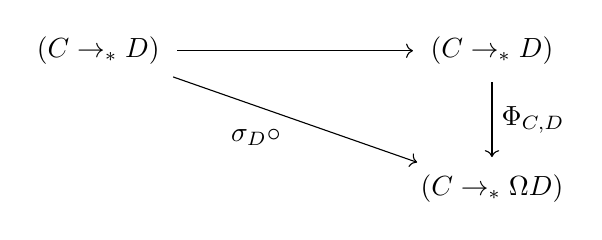
\begin{tikzpicture}[x=5cm,y=-1.75cm,baseline=(current bounding box.center)]
    \tikzset{arrow/.style={shorten >=0.1cm,shorten <=.1cm,->}}
    \node (A) at (0,0) {$(C \to_* D)$};
    \node (D) at (1,0) {$(\susp C \to_* \susp D)$};
    \node (C) at (1,1) {$(C \to_* \Omega \susp D)$};

    \draw[arrow] (A) to node [above] {$\susp$} (D);
    \draw[arrow] (A) to node [below left] {$\sigma_D \circ \, \blank$} (C);
    \draw[arrow] (D) to node [right] {$\Phi_{C,\susp D}$} (C);
    \end{tikzpicture}
    \end{equation}
\end{lem}
\begin{proof}
  By definition, for $f:C\ptdto D$, one has $\Phi \circ \susp (f) \jdeq
  \loopspace\null\susp(f)\circ \sigma_D$. Hence $\nat_\eta$ from
  \cref{prop:susp-loop-adjunction} provides the wanted witness of
  commutativity.
%%
%%  By easy calculation.\todo{We should do it!}
%%
%%  Denote $c_0$ and $d_0$ respectively for the distinguished point of $C$ and $D$.
%%  Let $f$ be a pointed function $C \ptdto D$ and let us show that the type
%%  $\susp (\Phi (f)) = \sigma_D \circ f$ is inhabited.
%%  %
%%  \todo[inline]{Really depends of the form we give to $\Phi$ and to the path pointing $\Phi(f)$!}
\end{proof}

The equivalence $\Phi$ also satisfies the following lemma:
\begin{lem} \label{lem:ap-Sigma}
    Let $X$ be a pointed type and $f : A \ptdto B$ be a pointed function.
    The following square commutes
    {\normalfont(}\kern-1pt up to homotopy{\normalfont)}:
    \begin{equation}
    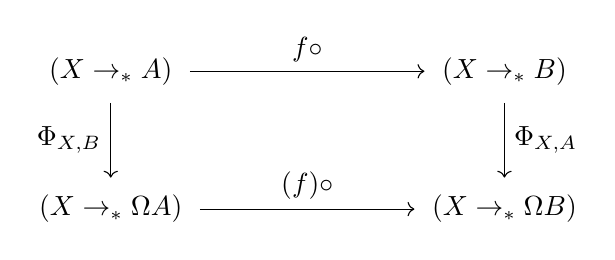
\begin{tikzpicture}[x=5cm,y=-1.75cm,baseline=(current bounding box.center)]
    \tikzset{arrow/.style={shorten >=0.1cm,shorten <=.1cm,->}}
    \node (A) at (0,0) {$(\susp X \to_* A)$};
    \node (D) at (1,0) {$(\susp X \to_* B)$};
    \node (B) at (0,1) {$(X \to_* \Omega A)$};
    \node (C) at (1,1) {$(X \to_* \Omega B)$};

    \draw[arrow] (A) to node [above] {$f \circ \blank$} (D);
    \draw[arrow] (A) to node [left] {$\Phi_{X,B}$} (B);
    \draw[arrow] (B) to node [above] {$\loopspace\null (f) \circ \blank$} (C);
    \draw[arrow] (D) to node [right] {$\Phi_{X,A}$} (C);
    \end{tikzpicture}
    \end{equation}
\end{lem}
\begin{proof}
    This is the content of \cref{def:wild-adj}.
    %
%%    By calculation.
%%    %  Starting with $f_0 : \susp X \to A$ and $f_1 : f_0(\north) = a_0$ and checking where this pair is mapped if we go first down and then right, we get:
%%    We start in the top left corner with $g_0 : \susp X \to A$ and $g_1 : g_0(\north) = a_0$. If we go first down, then right, we get the following, where we omit the proofs that the functions are pointed:
%%    \begin{equation}
%%    \begin{alignedat}{5}
%%    &\quad && g_0 : \susp X \to A & \\
%%    \mapsto &&& \lambda x. g_1 \cdot \ap {g_0}(\mrd(x_0)^{-1} \mrd(x)) \cdot g_1^{-1} : X \to \Omega A \\
%%    \mapsto &&& \lambda x. f_1 \cdot \ap {f_0}(g_1) \cdot  \ap {f_0 \circ g_0}(\mrd(x_0)^{-1} \mrd(x)) \cdot \ap {f_0}(g_1)^{-1} \cdot f_1^{-1} : X \to \Omega B
%%    \end{alignedat}
%%    \end{equation}
%%    If we go first right, then down, we get:
%%    \begin{equation}
%%    \begin{alignedat}{5}
%%    &\quad && g_0 : \susp X \to A & \\
%%    \mapsto &&&  f_0 \circ g_0 : \susp X \to B \\
%%    \mapsto &&& \lambda x. f_1 \cdot \ap {f_0}(g_1) \cdot  \ap {f_0 \circ g_0}(\mrd(x_0)^{-1} \mrd(x)) \cdot \ap {f_0}(g_1)^{-1} \cdot f_1^{-1} : X \to \Omega B
%%    \end{alignedat}
%%    \end{equation}
%%    The proofs that the functions are pointed are the canonical ones and coincide as well. (todo: if we have a formalisation, we can refer to that.) \todo{Pierre: this is the kind of stuff done in the HoTT-book that bug me a little}
\end{proof}

For a pointed type $A$, define the equivalence $\phi_A^n: (\Sn n \ptdto A) \to
\loopspace n A$ by induction on $n\geq 1$ as follows: for $n=1$,
$\phi_A^1(f:\Sc \ptdto A) \defequi \loopspace\null (f)(\Sloop)$ and for $n\geq
2$, $\phi^n \defequi \phi_{\loopspace\null A}^{n-1} \circ \Phi_{\Sn {n-1},A}$.
\begin{cor}\label{lem:iterated-ap-Sigma}
    For all $n \geq 0$ and $f$ as above, the diagram
    \begin{equation}
    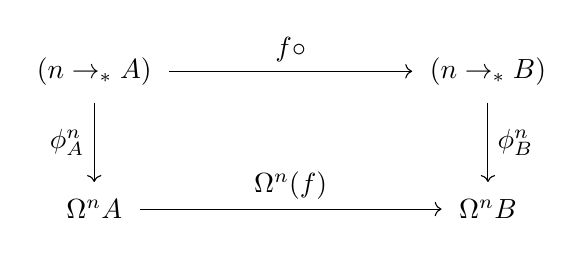
\begin{tikzpicture}[x=5cm,y=-1.75cm,baseline=(current bounding box.center)]
    \tikzset{arrow/.style={shorten >=0.1cm,shorten <=.1cm,->}}
    \node (A) at (0,0) {$(\Sn n \to_* A)$};
    \node (D) at (1,0) {$(\Sn n \to_* B)$};
    \node (B) at (0,1) {$\Omega^n A$};
    \node (C) at (1,1) {$\Omega^n B$};

    \draw[arrow] (A) to node [above] {$f \circ \blank$} (D);
    \draw[arrow] (A) to node [left] {$\phi_A^n$} (B);
    \draw[arrow] (B) to node [above] {$\Omega^n(f)$} (C);
    \draw[arrow] (D) to node [right] {$\phi_B^n$} (C);
    \end{tikzpicture}
    \end{equation}
    commutes.
\end{cor}
\begin{proof}
  By induction on $n:\NN$. For $n\defequi 1$, this is given by the wild functoriality of
  $\loopspace\null$ (see \cref{ex:loop-sus-wild-functors}):
  \begin{displaymath}
    \loopspace \null (f) (\phi^1 (g)) \jdeq \loopspace\null(f)(\loopspace\null(g)(\Sloop))
    =\loopspace\null(f\circ g)(\Sloop) \jdeq \phi^1(f\circ g)
  \end{displaymath}
  The step from $n$ to $n+1$ is an application of \cref{lem:ap-Sigma}.
\end{proof}


The above lemmas allow us to formulate a connection between the maps $\susp$ in
\eqref{eq:susp-monoid-morphism} and $\sigma_{\Sn n}$ in \eqref{eq:sigma}:
%, which will be needed in order to use \cref{thm:freudenthal} for \cref{thm:susp-is-monoid-iso}:

\begin{lem} \label{lem:sigma-susp}
  The maps $\sigma_{\Sn n}$ and $\susp$ are equal up to canonical isomorphism, i.e.\ the square
  \begin{equation} \label{eq:needs-to-commute}
    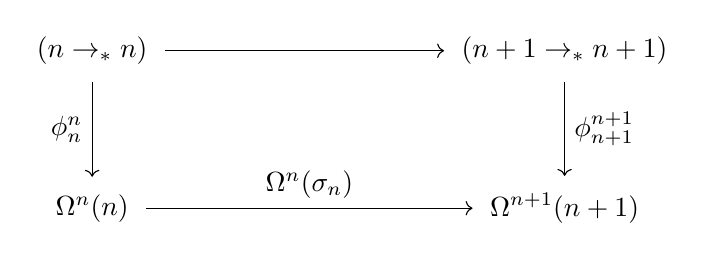
\begin{tikzpicture}[x=6cm,y=-2cm,baseline=(current bounding box.center)]
    \tikzset{arrow/.style={shorten >=0.1cm,shorten <=.1cm,->}}
    \node (A) at (0,0) {$(\Sn n \to_* \Sn n)$};
    \node (B) at (0,1) {$\Omega^n(\Sn n)$};
    \node (C) at (1,1) {$\Omega^{n+1}(\Sn {n+1})$};
    \node (D) at (1,0) {$(\Sn {n+1} \to_* \Sn {n+1})$};

    \draw[arrow] (A) to node [left] {$\phi_{\Sn n}^n$} (B);
    \draw[arrow] (B) to node [above] {$\Omega^n(\sigma_{\Sn n})$} (C);
    \draw[arrow] (D) to node [right] {$\phi_{\Sn {n+1}}^{n+1}$} (C);
    \draw[arrow] (A) to node [above] {$\susp$} (D);
    \end{tikzpicture}
  \end{equation}
  commutes.
\end{lem}
\begin{proof}%
  Recall that $\Sn {n+1} \jdeq \susp {\Sn n}$ and $\loopspace {n+1}(A) \jdeq
  \loopspace n (\loopspace\null A)$ for any pointed type $A$, so that we are
  free to use them interchangeably
  in the following diagram:
\begin{equation}
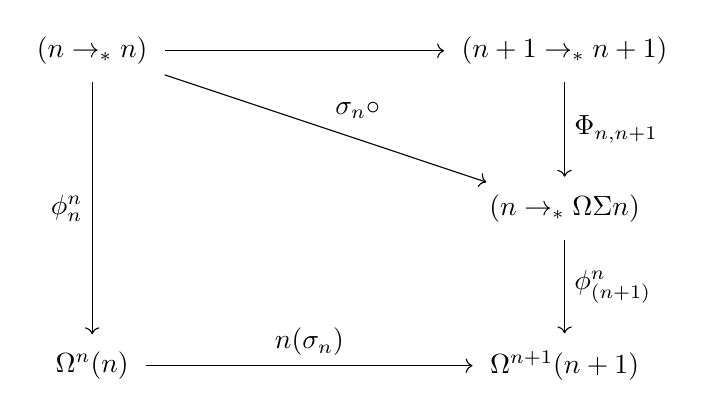
\begin{tikzpicture}[x=6cm,y=-2cm,baseline=(current bounding box.center)]
\tikzset{arrow/.style={shorten >=0.1cm,shorten <=.1cm,->}}
\node (A) at (0,0) {$(\Sn n \to_* \Sn n)$};
\node (B) at (0,2) {$\Omega^n(\Sn n)$};
\node (C) at (1,2) {$\Omega^{n+1}(\Sn {n+1})$};
\node (D) at (1,0) {$(\Sn {n+1} \to_* \Sn {n+1})$};
\node (E) at (1,1) {$(\Sn n \to_* \Omega \Sigma \Sn n)$};

\draw[arrow] (A) to node [left] {$\phi^n_{\Sn n}$} (B);
\draw[arrow] (B) to node [above] {$\loopspace n(\sigma_{\Sn n})$} (C);
%  \draw[arrow] (D) to node [right] {$\sim$} (C);
\draw[arrow] (A) to node [above] {$\susp$} (D);
\draw[arrow] (D) to node [right] {$\Phi_{\Sn n,\Sn {n+1}}$} (E);
\draw[arrow] (E) to node [right] {$\phi^n_{\loopspace\null(\Sn {n+1})}$} (C);
\draw[arrow] (A) to node [above right] {$\sigma_{\Sn n} \circ \blank$} (E);
\end{tikzpicture}
\end{equation}
The top triangle commutes by \cref{lem:adj-prop}.
The bottom quadrangle commutes by \cref{lem:iterated-ap-Sigma}.
\end{proof}

\cref{lem:sigma-susp} characterises the function \eqref{eq:susp-monoid-morphism}
in terms of $\sigma$.
Our motivation for this characterisation is that we know something about $\sigma$ through the following result:

\begin{thm}[{Freudenthal suspension theorem \cite[Thm 8.6.4]{HoTT}}] \label{thm:freudenthal}
    If $X$ is $n$-connected and pointed, with $n \geq 0$, then the map $\sigma_X$ is $2n$-connected. \qed
\end{thm}


Choosing $X$ to be $\Sn n$ and using that $\Sn n$ is $(n-1)$-truncated \cite[Corollary 8.2.2]{HoTT}, we get in particular the following instantiation:


\begin{cor} \label{cor:sigma-truncated}
For $n \geq 1$, the map
\begin{equation}
  \sigma_{\Sn n} : \Sn n \to \Omega(\Sn {n+1})
\end{equation}
is $2(n-1)$-truncated.
\end{cor}


To make use of this, we show how connectedness of functions interacts with loop spaces:

\begin{lem} \label{lem:conn-ap}
    Let $A$ and $B$ be types and $f : A \to B$ be a $k$-connected function ($k \geq -1$).
    For all $a_1, a_2 : A$, the function $\ap f : a_1 = a_2 \to f(a_1) = f(a_2)$ is $(k-1)$-connected.
\end{lem}
\begin{proof}
    Let us fix $a_1, a_2$, and $p : f(a_1) = f(a_2)$.
    We need to show that the fibre
    \begin{equation}
%        \higherTrunc {k-1} {\Sigma q : a_1 = a_2. \ap{f}(q) = p}
      \sum_{q : a_1 = a_2}\ap{f}(q) = p
    \end{equation}
    is $(k-1)$-connected.

%    By the connectedness assumption on $f$, the type $\higherTrunc k {f^{-1}(a_2)}$ is contractible.
    We consider the two elements
    $\highertrunc k {(a_1, p)}$
    and
    $\highertrunc k {(a_2, \refl {f(a_2)})}$ of
    the type $\higherTrunc k {f^{-1}(f(a_2))}$, which is contractible by the connectedness assumption on $f$.
    Therefore, the type of equalities between the two chosen elements is contractible as well.
    By \cite[Theorem 7.3.12]{HoTT}, this type of equalities is equivalent to
    \begin{equation} \label{eq:eq-in-truncated-fibre}
    \higherTrunc {k-1} {(a_1, p) = (a_2, \refl {f(a_2)})}.
    \end{equation}
    However,
%    the equality type $(a_1,p) = (a_2,\refl {f(a_2)})$ is
    this type is further equivalent to
    \begin{equation}
      \higherTrunc[\bigg] {k-1} {\sum_{q : a_1 = a_2} \ap f(q) = p},
    \end{equation}
    and the contractibility of this type is exactly what we had to show.
\end{proof}

By $k$-fold application of the above lemma, we get:
\begin{cor} \label{cor:n-2-connected}
    If $f : A \to_* B$ is $(k+m)$-connected with $k \geq 0$, $m \geq -2$, then
    $\Omega^k(f) : \Omega^k(A) \to \Omega^k(B)$ (viewed as a non-pointed function) is $m$-connected.

    Building on \cref{cor:sigma-truncated} we get that, for $n \geq 1$, the map
    \begin{equation}
      \loopspace n (\sigma_{\Sn n}) : \Omega^n(\Sn n) \to \Omega^{n+1}(\Sn {n+1})
    \end{equation}
    is $(n-2)$-connected.
    \qed
\end{cor}

We are now ready to restate and prove \cref{thm:susp-is-monoid-iso}:

\suspiso*
\begin{proof}
    Since identity and composition of the monoid structures are just given by the identity function and function composition,
    preservation of the monoid structure is just the (wild) functoriality of $\susp$.

    What is left to show is $0$-connectedness.
    In the commutative square of \cref{lem:sigma-susp}, the two vertical maps are equivalences and the bottom horizontal map is $(n-2)$-truncated by \cref{cor:n-2-connected}.
    This implies that the top horizontal map $\susp$ is $(n-2)$-connected as well.
    By assumption we have $(n-2) \geq 0$, which means that an $(n-2)$-connected map is also $0$-connected.
\end{proof}

\subsection{Connected components of
  \texorpdfstring{$\Sn n = \Sn n$}{Sn = Sn}}

Having shown \cref{thm:susp-is-monoid-iso}, we are now able to determine the number of connected components of symmetries of $\Sn n$.
Set-truncating a $0$-connected map gives an equivalences, and therefore:
\begin{cor}[{of \cref{thm:susp-is-monoid-iso}}] \label{cor:iso-of-monoids}
    For all $n \geq 2$, the map
    \begin{equation}
    \higherTrunc 0 {\susp} : \higherTrunc 0 {\Sn n \to_* \Sn n} \to \higherTrunc 0 {\Sn {n+1} \to_* \Sn {n+1}}
    \end{equation}
    is an isomorphism of monoids.\qed
\end{cor}

Recalling that we eventually want to reach non-pointed equivalences $\Sn n \simeq \Sn n$,
we want to remove the base points of the monoid morphism above.
We have the following general result:


\begin{lem} \label{lem:forget-points-conn}
    Let $X$ and $Y$ be types, and $x : X$ and $y : Y$ be points. If $Y$ is $n$-connected, then the canonical map which forgets the preservation of the base point $x$, given as
    \begin{alignat}{2}
    \pi_1: && \quad & ((X,x) \ptdto (Y,y)) \to (X \to Y) \\
    &&& (f,p) \mapsto f
    \end{alignat}
    is $(n-1)$-connected.
%    If $(X,x) \equiv (Y,y)$, then $\setTrunc{\pi_1}$ isomorphism of monoids.
\end{lem}
\begin{proof}
    Assume $f : X \to Y$.
    We calculate
    \begin{align}
      \pi_1^{-1}(f)
      &\weq \sum_{g : X \to Y}(g(x) = y) \times (g = f) \\
      &\weq f(x) = y, \label{eq:simplified-preimage}
    \end{align}
    where we use that the dependent pair type $\sum_{g : X \to Y} (g = f)$ is contractible.
    Since $Y$ is $n$-connected, the type \eqref{eq:simplified-preimage} is $(n-1)$-connected by \cref{lem:conn-ap}.
%
%    \begin{alignat}{2}
%    &&& \setTrunc{\Sigma(f : X \to X). f(x) = x} \\
%    &\simeq &\quad & \setTrunc{\Sigma(f : X \to X). \setTrunc{f(x) = x}} \\
%    &\simeq && \setTrunc{X \to X},
%    \end{alignat}
%    where the first steps holds by \cite[Thm.~7.3.9]{HoTT} and the second by the connectedness assumption.
%    Composition and identities are preserved by the projection $\pi_1$, and thus also by $\setTrunc{\pi_1}$.
\end{proof}

Using that every $\Sn n$ (for $n \geq 2$) is $1$-connected, the case $(X,x) \equiv (Y,y) \equiv (\Sn n, \north)$ gives the following:
%\begin{cor} \label{cor:forget-point-iso}
%    If $X$ is a $1$-connected type and $x:A$, then
%    \begin{alignat}{2}
%    \setTrunc{\pi_1}: && \quad & \setTrunc{(X,x) \ptdto (X,x)} \to \setTrunc{X \to X} \\
%    &&& \highertrunc 0 {(f,p)} \mapsto \highertrunc 0 f
%    \end{alignat}
%    is an isomorphism of monoids.
%\end{cor}
%\begin{proof}
%    The monoid structure is clearly preserved, and a $0$-connected map becomes an equivalence when $0$-truncating.
%\end{proof}
%
%Since every $\Sn n$ (for $n \geq 2$) is $1$-connected, this allows us to get rid of the preservation of base points in \cref{cor:iso-of-monoids}:

\begin{cor} \label{cor:higher-spheres-2-comp}
    For all natural numbers $n \geq 2$, the map
    \begin{equation}
    \higherTrunc 0 {\susp} : \higherTrunc 0 {\Sn n \to \Sn n} \to \higherTrunc 0 {\Sn {n+1} \to \Sn {n+1}}
    \end{equation}
    is an isomorphism of monoids.
\end{cor}
\begin{proof}
    The monoid structure is clearly preserved, and the map is $0$-connected by the lemma. A $0$-connected map becomes an equivalence when $0$-truncating domain and codomain.
\end{proof}

Recall that we are ultimately interested in the group $\setTrunc{\Sn n = \Sn n}$ and not in the monoid $\setTrunc{\Sn n \to \Sn n}$ itself. The following result states that the former is the group of invertible elements of the latter.
\begin{lem}
    Let $A$ be a type. The type of invertible elements in the monoid $\setTrunc{A \to A}$
    is the (essential) image of the induced inclusion $i:\setTrunc{A \weq A} \to
    \setTrunc{A \to A}$.
    \label{lemma:invertible-truncated-Sn-pointed-weq}
\end{lem}
\begin{proof}
    Obviously, the truncation $\settrunc{f}$ of an equivalence $f$ is invertible,
    as $\settrunc{\inv f}$ is an inverse for it.

    Conversely, if $x:\setTrunc{A \to A}$ is invertible, then
    it has a unique inverse $\inv x$, and we want to
    produce an element of the type:
    \begin{displaymath}
    \sum_{y:\setTrunc{A \weq A}} x = i(y)
    \end{displaymath}
    %
    As $x=i(y)$ is a proposition for every $y$ in the set $\setTrunc{A
        \weq A}$, this type is a set itself. Hence, one might assume
    that $x \jdeq \settrunc f$ for some function $f:A \to A$ as well
    as its inverse $\inv x \jdeq \settrunc g$ for some $g:A \to A$.
    %
    From the inverse law in the monoid $\setTrunc{A \to A}$, one
    derives that both $fg$ and $gf$ are merely equal to $\id_{A}$. To prove
    the proposition that $f$ is an equivalence, one can then assume actual
    witnesses of $fg=\id_{A}$ and $gf=\id_{A}$. Then $g$ is a
    pseudo-inverse for $f$, which solves the problem.
\end{proof}

We now see that there are two connected components of symmetries of spheres:
\begin{thm} \label{thm:higher-spheres-2}
    For any $n \geq 1$, we have an equivalence of types
    \begin{equation}
    \higherTrunc 0 {\Sn n= \Sn n} \weq \bn 2
    \end{equation}
\end{thm}
\begin{proof}
  For $n = 1$ and $n=2$, we have established this result in the previous
  sections (see \cref{thm:symmetries-of-S1} and
  \cref{prop:symm-S2-connected-components}).  For higher $n$, it follows by
  induction on $n$ with the help of \cref{cor:higher-spheres-2-comp} that the
  monoids $\setTrunc{\Sn n \to \Sn n}$ have exactly two invertible elements.
  Then \cref{lemma:invertible-truncated-Sn-pointed-weq} allows us to conclude.
\end{proof}

\subsection{Concrete symmetries of \texorpdfstring{$\Sn n$}{Sn}}

As in the cases of $\Sc$ and $\Sp$, we want to construct one concrete element for each of the two connected components of symmetries on $\Sn n$ that were established in \cref{thm:higher-spheres-2}.
As before, these two elements are given as $\id$ and $-\id : \Sn n \to \Sn n$.
It is clear that they are symmetries (i.e.\ equivalences), as each is self-inverse.
What is less obvious is that they are distinguishable, i.e.\ represent the two different components in \cref{thm:higher-spheres-2} rather than the same.
Instead of showing $\id \neq -\id$ as in \cref{lemma:S2-id-neq-minusid}, we show that suspension and ``negation'' commute in \cref{lem:susp-neg-commute}.

In this subsection, we annotate the constructors of the suspension with their type in order to avoid ambiguity.
For example, for any type $A$, we have $-\id_A : \susp(A) \to \susp(A)$ defined by
$\north_{\susp(A)} \mapsto \south_{\susp(A)}$,
$\south_{\susp(A)} \mapsto \north_{\susp(A)}$,
and $\mrd_{\susp(A)}(a) \mapsto \inv{\mrd_{\susp(A)}(a)}$.
For $f : A \to B$, we have $\susp(f) : \susp(A) \to \susp(B)$ given by $\north_{\susp(A)} \mapsto \north_{\susp(B)}$,
$\south_{\susp(A)} \mapsto \south_{\susp(B)}$,
and $\mrd_{\susp(A)}(a) \mapsto \mrd_{\susp(B)}(f(a))$.
Notice that the index of $\mrd$ is redundant when applied to an argument as its type is then inferrable from the type of the argument. We shall then use $\mrd(a)$ instead of $\mrd_{\susp(A)}(a)$ for $a:A$ whenever it make the text more readable.
Moreover, we use colours to make the connections between formulas and diagrams easier to identify.

\begin{lem} \label{lem:susp-neg-commute}
	For any type $A$, the two functions $\susp(-\id_{\susp(A)})$ and $-\id_{\susp(\susp(A))}$ of type $\susp(\susp(A)) \to \susp(\susp(A))$ are equal.
\end{lem}
A proof of this lemma is available in cubical Agda~\cite{doublesusp}.
Here, we give the argument in the style of \cite{HoTT}:
\begin{proof}
  \def\cg{\color{darkgreen}}
  \def\cb{\color{darkblue}}
  Using function extensionality and assuming $x : \susp\susp A$,
  we need to construct $h(x)$ of type
  $T(x) \defequi ( \susp(-\id_{\susp A})(x) = -\id_{\susp{\susp A}}(x) )$.
  We do induction on $x$ and define:
  \begin{alignat}{2}
    \cg h(\north_{\susp\susp A})
    & \cg \defequi \mrd(\north_{\susp A})
    && \cg : \south_{\susp\susp A} = \south_{\susp\susp A}
    \label{eq:green}
    \\
    \cb h(\south_{\susp\susp A})
    & \cb \defequi \inv{\left(\mrd(\south_{\susp A})\right)}
    && \cb : \south_{\susp\susp A} = \north_{\susp\susp A}
    \label{eq:blue}
  \end{alignat}

  The last component to be defined is, for all $y : \susp A$,
  a higher path $\ap h(\mrd(y))$ whose type is
  $\pathover {h(\north_{\susp\susp A})} T {\mrd(y)} {h(\south_{\susp\susp A})}$.
	After rewriting path-overs as path composition using \cite[Lem~2.11.3]{HoTT},
  the type of this component is equivalent to the the type of commutativity proofs for the square:
	\begin{equation}\label{eq:y-commute}
	\begin{tikzpicture}[x=6.5cm,y=-2cm,baseline=(current bounding box.center)]
	\node[text=darkgreen] (N1) at (0,0) {$\north_{\susp\susp A}$};
	\node[text=darkgreen] (S1) at (0,1) {$\south_{\susp\susp A}$};
	\node[text=darkblue] (S2) at (1,0) {$\south_{\susp\susp A}$};
	\node[text=darkblue] (N2) at (1,1) {$\north_{\susp\susp A}$};
	\draw[->,text=darkgreen] (N1) to node[left] {$\mrd(\north_{\susp A})$} (S1);
        \draw[->,text=darkblue] (S2) to node[right] {$\inv{\mrd(\south_{\susp A})}$} (N2);
	\draw[->] (N1) to node[above] {$\mrd(-\id_{\susp A}(y))$} (S2);
        \draw[->] (S1) to node[above] {$\inv{\mrd(y)}$} (N2);
	\end{tikzpicture}
	\end{equation}
	To simplify the presentation, we write
	\begin{align}
	N & \defequi \north_{\susp \susp A} \\
	S & \defequi \south_{\susp \susp A} \\
	m_N & \defequi \mrd(\north_{\susp A}) \\
	m_S & \defequi \mrd(\south_{\susp A})
	\end{align}
	We do induction on $y$.
	For $y \equiv \north_{\susp A}$, after simplifying (normalising) the terms, the square \eqref{eq:y-commute} becomes
	\begin{equation}\label{eq:N-commute}
	\begin{tikzpicture}[x=6.5cm,y=-2cm,baseline=(current bounding box.center)]
	\node[text=darkgreen] (N1) at (0,0) {$N$};
	\node[text=darkgreen] (S1) at (0,1) {$S$};
	\node[text=darkblue] (S2) at (1,0) {$S$};
	\node[text=darkblue] (N2) at (1,1) {$N$};
	\draw[->,text=darkgreen,color=darkgreen] (N1) to node[left] {$m_N$} (S1);
        \draw[->,text=darkblue,color=darkblue] (S2) to node[right] {$\inv{m_S}$} (N2);
	\draw[->] (N1) to node[above] {$m_S$} (S2);
        \draw[->] (S1) to node[above] {$\inv{m_N}$} (N2);
	\end{tikzpicture}
	\end{equation}
        with the obvious commutativity proof $c(m_S,m_N) : \inv{m_S} \cdot {m_S} = \inv{m_N} \cdot {m_N}$. (Given $p$, $q$, we define $c(p,q) : \inv{p}\cdot p = \inv{q}\cdot q$ by path induction on $p$ and $q$ such that $c(\refl{},\refl{}) \jdeq \refl{}$.)
%	 : m_N \cdot \inv{m_N} = m_S \cdot \inv{m_S}$.
	Similarly, for $y \equiv \south_{\susp A}$, the square \eqref{eq:y-commute} becomes
	\begin{equation}\label{eq:S-commute}
	\begin{tikzpicture}[x=6.5cm,y=-2cm,baseline=(current bounding box.center)]
	\node[text=darkgreen] (N1) at (0,0) {$N$};
	\node[text=darkgreen] (S1) at (0,1) {$S$};
	\node[text=darkblue] (S2) at (1,0) {$S$};
	\node[text=darkblue] (N2) at (1,1) {$N$};
	\draw[->,text=darkgreen,color=darkgreen] (N1) to node[left] {$m_N$} (S1);
        \draw[->,text=darkblue,color=darkblue] (S2) to node[right] {$\inv{m_S}$} (N2);
	\draw[->] (N1) to node[above] {$m_N$} (S2);
        \draw[->] (S1) to node[above] {$\inv{m_S}$} (N2);
	\end{tikzpicture}
	\end{equation}
        with the trivial commutativity proof $\refl{} : \inv{m_S} \cdot {m_N} = \inv{m_S} \cdot m_N$.

	Finally, we consider the third case of the induction on $y$, namely the case that $y$ is a path of the form $\mrd(z)$ for some $z : A$.
        In this case, we need to find an element of the pathover type $\pathover {c(m_S,m_N)} U {\mrd(z)} \refl{}$ where the type family $U$ is given by:
        \begin{displaymath}
          U(y) \defequi \left( \inv{m_S} \cdot \mrd(-\id_{\susp A}(y)) = \inv{\mrd(y)} \cdot m_N\right)
        \end{displaymath}
        In other words, one needs to show an equality between the ``fillers'' of the two squares \eqref{eq:N-commute} and \eqref{eq:S-commute}, and this equality lies over $\mrd(z)$ in the type family $U$ given at each point $y$ by square~\eqref{eq:y-commute}.
%%      (i.e.\ depends on) the two equalities that stem from the top horizontal arrow and the bottom horizontal arrow in \eqref{eq:y-commute} (note that the two vertical arrows in \cref{eq:y-commute} do not depend on $y$).
        We first need to understand transport in $U$ over a path $p$ in $\susp A$. %
        The intuition is that the top and bottom arrows of square~\eqref{eq:y-commute}
        can be deformed by $p$ while the vertical arrows remain constant.
        This suggests that the transport of $c:U(y)$ over $p:y=y'$ is given by:
        \begin{displaymath}
          \ap {\blank \cdot m_N} (\ap {\inv{} \circ \mrd} (p))
          \cdot c \cdot
          \inv{\left( \ap{\inv{m_S} \cdot \blank} (\ap {\mrd \circ -\id_{\susp A}} (p)) \right)}
          : U(y')
        \end{displaymath}
 %\todo[inline]{One can use whiskering here if you find it easier to parse.}
        Formally this follows again from \cite[Lem~2.11.3]{HoTT},
        to be proved by path induction over $p$, the case for $p\jdeq \refl y$ being
        given by standard path algebra.
        We now instantiate this transport with $p \jdeq \mrd(z)$ for $z:A$. Write:
        \begin{alignat}{2}
	\alpha &\defequi \ap{\mrd}\left(\ap{-\id_{\susp A}}(\mrd(z))\right) && : m_S=m_N
        \label{eq:alpha-def}
        \\
        \beta &\defequi \ap\mrd(\mrd(z)) && : m_N=m_S
        \label{eq:beta-def}
	\end{alignat}
	Then the transport of $c(m_S,m_N)$, the filler of square (\ref{eq:N-commute}),
        is given by the composition
	\begin{equation}\label{eq:first-square-composed}
          \ap{(\blank\cdot {\color{darkgreen}m_N})\circ{}^{-1}}(\beta) \cdot c(m_S,m_N) \cdot
                            \ap{{\color{blue}\inv{m_S}}\cdot\blank}(\inv{\alpha})
	\end{equation}
	of type ${\color{blue}\inv{m_S}} \cdot m_N = \inv{m_S} \cdot {\color{darkgreen}m_N}$.
	The situation can be depicted as follows:
	\begin{equation}\label{eq:N-commute-with-ears}
	\begin{tikzpicture}[x=6.5cm,y=-2cm,baseline=(current bounding box.center)]
	\node[text=darkgreen] (N1) at (0,0) {$N$};
	\node[text=darkgreen] (S1) at (0,1) {$S$};
	\node[text=darkblue] (S2) at (1,0) {$S$};
	\node[text=darkblue] (N2) at (1,1) {$N$};
	\draw[->,text=darkgreen,color=darkgreen] (N1) to node[left] {$m_N$} (S1);
	\draw[->,text=darkblue,color=darkblue] (S2) to node[right] {$\inv{m_S}$} (N2);
	\draw[->] (N1) to node[above] {$m_S$} (S2);
	\draw[->] (S1) to node[above] {$\inv{m_N}$} (N2);
	\draw[->, bend left = 60] (N1) to node[above] {$m_N$} (S2);
	\draw[<-, bend left = 60] (N2) to node[above] {$\inv{m_S}$} (S1);
	%\node[] (A) at (0.5,.5) {$c(m_S,m_N)$};
	\node[] (phantom1) at (.5,-1.0) {};
	\node[] (phantom2) at (.5,-.1) {};
	\node[] (phantom3) at (.5,0.9) {};
	\node[] (phantom4) at (.5,1.85) {};
	\draw[->,cell] (phantom2) to node[left] {$\alpha$} (phantom1);
	\draw[->,cell] (phantom3) to node[right] {$\ap{\inv{}}\beta$} (phantom4);
        \draw[->,cell, shorten >=3em, shorten <=3em] (S2) to node[midway,fill=white]{$c(m_S,m_N)$} (S1);
	\end{tikzpicture}
	\end{equation}
  The goal is now to show that \eqref{eq:first-square-composed}
  is equal to the trivial proof $\refl{}$
  filling square~\eqref{eq:S-commute},
  the outer `square' of (\ref{eq:N-commute-with-ears}).
  Unfolding the definition of $-\id_{\susp A}$ in~\eqref{eq:alpha-def}
  and using standard path algebra steps,
  we get $\alpha = \inv{\beta}$,
  and then this task simplifies to showing that the following diagram commutes:
  \begin{equation}\label{eq:3-cell}
  \begin{tikzcd}[column sep=6em,labels={font=\normalsize}]
    m_N^{-1}\cdot {\color{darkgreen}m_N}
      \arrow[Rightarrow, swap]{dd}{\ap{(\blank\cdot {\color{darkgreen}m_N})\circ\inv{}}(\beta)}
      \arrow[Leftarrow]{rr}{c(m_S,m_N)}&&
    {\color{blue}\inv{m_S}}\cdot m_S
      \arrow[Leftarrow, swap]{dd}{\ap{{\color{blue}\inv{m_S}}\cdot\blank}(\beta)}
 \\\\
    \inv{m_S}\cdot {\color{darkgreen}m_N}
       \arrow[Leftarrow, swap]{rr}{\refl{}} &&
    {\color{blue}\inv{m_S}}\cdot m_N
  \end{tikzcd}
  \end{equation}


  The easiest way to show that (\ref{eq:3-cell}) commutes
  is to generalise to arbitrary points $N$, $S$
  and arbitrary paths $m_N,m_S : N=S$,
  as well as to an arbitrary higher path $\beta: m_N=m_S$.
  One starts by doing path induction on $m_N$,
  reducing the task to the case $S\jdeq N$ and $m_N\jdeq \refl N$,
  and arbitrary $m_S:N=N$ and $\beta: m_N = m_S$.
  One can then do path induction on $\beta$,
  reducing the task to the case $m_S\jdeq m_N$
  and $\beta \jdeq \refl{m_N}$.
  But now, as $m_N \jdeq \refl N$, all paths appearing in the diagram,
  including $c(m_S,m_N)$, are reflexivity paths.
  Hence we can conclude by simple path algebra.
\end{proof}


\begin{rem}
	In cubical type theory, the problem of proving an equality between the squares \eqref{eq:N-commute} and \eqref{eq:S-commute} naturally becomes the problem of filling the following cube:

	\begin{equation}\label{eq:ulriks-cube}
	\begin{tikzpicture}[x=6.5cm,y=-3cm,baseline=(current bounding box.center)]
	\node[text=darkgreen] (N1F) at (0,0) {$N$};
	\node[text=darkgreen] (S1F) at (0,1) {$S$};
	\node[text=darkblue] (S2F) at (1,0) {$S$};
	\node[text=darkblue] (N2F) at (1,1) {$N$};

	\node[text=darkgreen] (N1B) at (-.3,-.3) {$N$};
	\node[text=darkgreen] (S1B) at (-.3,.7) {$S$};
	\node[text=darkblue] (S2B) at (.7,-.3) {$S$};
	\node[text=darkblue] (N2B) at (.7,.7) {$N$};


	\draw[tikzbackground,text=darkgreen,color=darkgreen] (N1B) to node[left] {$m_N$} (S1B);
	\draw[tikzbackground,text=darkblue,color=darkblue] (N2B) to node[right] {$m_S$} (S2B);
	\draw[tikzbackground] (N1B) to node[above] {$m_N$} (S2B);
	\draw[tikzbackground] (N2B) to node[above] {$m_S$} (S1B);

	\draw[tikzequal,color=darkgreen] (N1F) to node {} (N1B);
	\draw[tikzequal,color=darkblue] (N2F) to node {} (N2B);
	\draw[tikzequal,color=darkgreen] (S1F) to node {} (S1B);
	\draw[tikzequal,color=darkblue] (S2F) to node {} (S2B);

	\draw[tikzforeground,text=darkgreen,color=darkgreen] (N1F) to node[left] {$m_N$} (S1F);
	\draw[tikzforeground,text=darkblue,color=darkblue] (N2F) to node[right] {$m_S$} (S2F);
	\draw[tikzforeground] (N1F) to node[above] {$m_S$} (S2F);
	\draw[tikzforeground] (N2F) to node[above] {$m_N$} (S1F);

	\end{tikzpicture}
	\end{equation}
	The front square is \eqref{eq:N-commute}, the back square is \eqref{eq:S-commute},
        the left and right are $\refl{}$, the top is $\alpha$, and the bottom is $\beta$,
        each appropriately oriented.
	The colours indicate the squares that came from the
        definitions in \eqref{eq:green} and \eqref{eq:blue}.
\end{rem}


\begin{cor}\label{cor:id-not-minus-id}
	For any $n \geq 1$, we have $\id_{\Sn n} \neq -\id_{\Sn n}$, and any symmetry of $\Sn n$ is merely equal to either $\id_{\Sn n}$ or $-\id_{\Sn n}$.
\end{cor}
\begin{proof}
	We know the statement for $n \equiv 1$ and $n \equiv 2$ from the previous sections.
	The rest is done by induction on $n$, so we assume $\id_{\Sn n} \neq -\id_{\Sn n}$.
	By
	\cref{cor:higher-spheres-2-comp}, we have $\susp(\id_{\Sn n}) \neq \susp(-\id_{\Sn n})$.
	As $\id_{\Sn {n+1}} = \susp(\id_{\Sn n})$ trivially holds and
	we further have $-\id_{\Sn {n+1}} = \susp(-\id_{\Sn n})$
	by \cref{lem:susp-neg-commute}, the claimed inequality follows.
	Therefore, the two symmetries lie in different components, and any symmetry lies in one of the two components given by \cref{thm:higher-spheres-2}.
\end{proof}

\section{The structure of the components}
\label{sec:structure-components}

\subsection{Interlude on Whitehead products}
\label{sec:whitehead-interlude}

Before focusing on the components of $\Sn n = \Sn n$,
we'll need a few general results on Whitehead products.

We recall a few standard operations on types that can be constructed using pushouts. The \emph{pushout} of a span $A \stackrel f\leftarrow C \stackrel g\to B$ is the higher inductive type $D$ defined by
\begin{itemize}
\item two maps $\inl : A \to D$ and $\inr : B \to D$, and
  a dependent function $\glue : \prod_{x:C} \inl(f(x)) = \inr(g(x))$
\end{itemize}
with the following induction rule:
\begin{quote}
  given a type family $T\from D \to \UU$, every
  triple of elements
  \begin{displaymath}
    \ell\from \prod_{a\from A}T(\inl(a)), \quad
    r\from \prod_{b\from B}T(\inr(b)), \quad
    p\from \prod_{x\from C}\pathover {\ell(f(x))} T {\glue\,x} {r(g(x))}
  \end{displaymath}
  defines a dependent function
  \begin{displaymath}
    \ind(\ell,r,p)\from\prod_{x\from D} T(x)
  \end{displaymath}
  such that
  \begin{gather*}
    \ind(\ell,r,p)(\inl\,a) \jdeq \ell(a), \quad
    \ind(\ell,r,p)(\inr\,b) \jdeq r(b),\\
    \ap{\ind(\ell,r,p)}(\glue x) = p(x)\ \text{for all}\ x\from C.
  \end{gather*}
\end{quote}
The rules for the pushout ensure that we have a commutative square
\[
  \begin{tikzcd}
    C \ar[r,"g"]\ar[d,"f"']\ar[pushout] & B \ar[d,"\inr"] \\
    A \ar[r,"\inl"'] & D,
  \end{tikzcd}
\]
and any other commutative square with the same span induces a unique
map from $D$.  If the induced map is an equivalence, then we say the
square is a \emph{pushout square}.

The other higher inductive types we've used so far, the circle, suspensions,
and truncations, can all be defined in terms of pushouts. For example, the
suspension $\susp A$ is equivalent to the pushout of the unique span $1
\leftarrow A \to 1$.

Another instance of such a pushout construction is the \emph{join} $A * B$ of
two types $A$ and $B$, defined as the pushout of the product projections:
\begin{equation}
  \begin{tikzcd}
    A \times B \ar[r,"\snd"]\ar[d,"\fst"']\ar[pushout] & B \ar[d,"\inr"] \\
    A \ar[r,"\inl"'] & A * B
  \end{tikzcd}
\end{equation}
Notice that if $A$ is pointed at a point $a_0$, then we make the join $A*B$ a
type pointed at $\inl(a_0)$.
\begin{lem}
  Let $A$ and $B$ be pointed types, repectively pointed at $a_0$ and  $b_0$.
  Then, for every pointed type $X$, there is an equivalence of type:
  \begin{equation}
    (A \ptdto (B \ptdto \loopspace{}X)) \weq (A*B \ptdto X)
    \label{eq:UMP-join-loopspace-version}
  \end{equation}
  \label{lemma:UMP-join-vs-loopspace}
\end{lem}
\begin{proof}
  Given $f: A \ptdto (B \ptdto \loopspace{}X)$, construct $\bar f:A*B \ptdto X$
  by induction:
  \begin{equation}
    \begin{aligned}
      \bar f(\inl(a)) &\defequi x_0 \quad \text{for $a:A$} \\
      \bar f(\inr(b)) &\defequi x_0 \quad \text{for $b:B$} \\
      \ap{\bar f}(\glue(a,b)) &\defis f(a)(b) \quad \text{for $a:A,b:B$}
    \end{aligned}
    \label{eq:def-barf-from-join-UMP}
  \end{equation}
  The map $\bar f$ is trivially pointed.

  This construction $f\mapsto \bar f$ admits an inverse. Indeed, as $A$ and $B$
  are both pointed, for any $a:A$ and $b:B$, one has a an element $\tau_{a,b}$
  of $\loopspace{}(A*B)$ constructed as the following composition of paths:
  \begin{equation}
    \begin{tikzcd}[column sep=large]
      \inl(a_0) \rar["{\glue(a_0,b_0)}"] & \inr(b_0) \rar["\inv{\glue(a,b_0)}"]
      & \inl(a) \rar["{\glue(a,b)}"] & \inr(b) \rar["\inv{\glue(a_0,b)}"]
      & \inl(a_0)
    \end{tikzcd}
    \label{eq:def-tau-ab}
  \end{equation}
  Then, to any $g:A*B \ptdto X$, one can map the function $\hat g: a \mapsto
  (b\mapsto \loopspace\null(g)(\tau_{a,b}))$.
  The map $\hat g$ is a pointed, as
  $\tau_{a_0,b} = \tau_{a,b_0} = \refl{\inl(a_0)}$ for all $a:A$ and $b:B$
  by path algebra.
  The construction $g
  \mapsto \hat g$ provides an inverse to $f \mapsto \bar f$.
  A proof of this has been formalized in cubical Agda~\cite{joinloopadj}.
  There, it's also checked that this equivalence arises from
  a wild adjunction, cf.~\cref{prop:join-loop-adjunction}.
\end{proof}

Finally, the \emph{wedge sum} $A \vee B$ of pointed types $A$ and $B$, with
respective distinguished points $a_0$ and $b_0$, is the pushout of the
point inclusions:
\[
  \begin{tikzcd}
    1 \ar[r,"b_0"]\ar[d,"a_0"']\ar[pushout] & B \ar[d,"\inr"] \\
    A \ar[r,"\inl"'] & A \vee B
  \end{tikzcd}
\]
This is a pointed type, with point $\inl(a_0)$.
%
There is a (pointed) map $i : A \vee B \to A \times B$, called \emph{wedge
inclusion}, defined by $i(\inl a) \jdeq (a , b_0)$, $i(\inr b) \jdeq (a_0, b)$,
and $\ap{i}(\glue\ast) = \refl{(a_0,b_0)}$ (where $\ast$ is the unique element
of $1$).

For the rest of this section we fix two pointed types $A$ and $B$, and we
denote $a_0$ and $b_0$ the base points of $A$ and $B$.
We repeat here the definition of the generalized Whitehead product
from \cite[Sec.~3.3]{brunerie:thesis}.
\begin{defi}
  There is a map $W = W_{A,B} : A * B \to \susp A \vee \susp B$
  making a pushout square with the wedge inclusion $i$:
  \begin{equation}\label{eq:def-join-wedge-pushout}
    \begin{tikzcd}
      A * B \ar[r,"W"]\ar[d]\ar[pushout] & \susp A \vee \susp B\ar[d,"i"] \\
      1 \ar[r] & \susp A \times \susp B
    \end{tikzcd}
  \end{equation}
  We have $W(\inl a) \jdeq \inr N$, $W(\inr b) \jdeq \inl N$,
  and
  \[
    \ap{W}(\glue(a,b)) = \ap{\inl}(\sigma_A(a))
    \cdot (\glue\ast)^{-1} \cdot \ap{\inr}(\sigma_B(b)).
  \]
  The map $W_{A,B}$ is pointed by the path $\inv{(\glue \ast)} : W(\inl(a_0))
  \jdeq \inr(\north) = \inl(\north)$.
\end{defi}
The fact that \eqref{eq:def-join-wedge-pushout} is a pushout square is
deduced using the $3{\times}3$-lemma in \cite[Prop.~3.3.2]{brunerie:thesis}.
However, this fact plays no role in our arguments below.

We now also fix another pointed type $X$, with distinguished point $x_0$.
\begin{defi}
  \label{defn:gen-Whitehead-product}
  The generalized Whitehead product of $\alpha : \susp A \ptdto X$
  and $\beta : \susp B \ptdto X$
  is the composition
  \[
    [\alpha, \beta] \defeq (\alpha \vee \beta) \circ W_{A,B}
    : A * B \ptdto X.
  \]
\end{defi}
If $A\jdeq \Sn p$ and $B\jdeq\Sn q$,
then $A * B \weq \Sn{p+q+1}$~\cite[Prop.~1.8.8]{brunerie:thesis},
so one can obtain a map
\begin{equation}\label{eq:whitehead-product}
  [\blank,\blank] : \hgr {p+1}(X) \times \hgr {q+1}(X) \to \hgr{p+q+1}(X),
\end{equation}
which is the usual Whitehead product on homotopy groups. Explicitely, given
$a:\hgr {p+1} (X)$ and $b:\hgr {q+1} (X)$, one wants to define the element
$[a,b]$ of the set $\hgr {p+q+1} (X)$. As we are targeting a set, one can as
well assume $a \jdeq \settrunc{\alpha}$ and $b \jdeq \settrunc{\beta}$ for
$\alpha:\loopspace{p+1}(X)$ and $\beta:\loopspace{q+1}(X)$. Using the
equivalences
\begin{equation}
  \loopspace{p+1}(X) \weq \susp\Sn {p} \ptdto X, \quad
  \loopspace{q+1}(X) \weq \susp\Sn {q} \ptdto X,
  \label{eq:equiv-loopspace-map-from-sphere-whitehead}
\end{equation}
one gets pointed maps, abusively denoted again $\alpha: \susp \Sn {p} \ptdto
X$ and $\beta: \susp \Sn {q} \ptdto X$. The element $[a,b] : \hgr{p+q+1}(X)$ is then
defined as $\settrunc{[\alpha,\beta]}$ (where $[\alpha, \beta]$ is defined
following \cref{defn:gen-Whitehead-product}).

Fix now a pointed map $\beta : \susp B \ptdto X$, whose pointing path is
$\beta_0:\beta(\north) = x_0$, and consider the evaluation fiber sequence
\[
  \conncomp{(\susp B \ptdto X)}{\beta}
  \ptdto \conncomp{(\susp B \to X)}{\beta}
  \ptdto X.
\]
(It's not necessary to take connected components.
Doing so allows us to emphasize the base points of the various function types.)

Let us consider the associated long exact sequence
\[
  \begin{tikzcd}
    \cdots \ar[r]\ar[d,phantom, "\partial_\beta"{xshift=-8ex,yshift=1ex}] &
    \pi_{n+1}(\susp B \to X, \beta) \ar[r] \ar[d, phantom, ""{coordinate, name=Z}] &
    \pi_{n+1}(X) \ar[dll, rounded corners,
    to path={ -- ([xshift=8.5ex]\tikztostart.center)
      |- (Z) [near end]\tikztonodes
      -| ([xshift=-13ex]\tikztotarget.center) -- (\tikztotarget)}] \\
    \pi_n(\susp B \ptdto X,\beta) \ar[r] &
    \pi_n(\susp B \to X,\beta) \ar[r] &
    \cdots
  \end{tikzcd}
\]
We wish to express the connecting homomorphism $\partial_\beta$ at $n\ge0$
in terms of the generalized Whitehead product.
%
\newcommand{\wunit}{1} %unit in wild group
%
In order to do so, we will reason about the map $\delta_\beta: (\susp \Sn n \ptdto X)
\to (\Sn n \ptdto \conncomp{(\susp B \ptdto X)}\beta)$ such that
\begin{equation}
  \Trunc[\big]{
    \phi_{\conncomp{(\susp B \ptdto X)}\beta}^n \circ
    \delta_\beta \circ
    \inv{\left( \phi_X^{n+1} \right)}
  }_0
  = \partial_\beta.
  \label{eq:def-delta-beta}
\end{equation}
We are going to construct a commuting square of the following form:
\begin{equation}\label{eq:Whitehead-special}
  \begin{tikzcd}
    (\susp{\Sn n} \ptdto X)
    \ar[r,"\delta_\beta"] \ar[d,"\rho_\beta"'] &
    (\Sn n \ptdto \conncomp{(\susp B \ptdto X)}{\beta})
    \ar[d,"\xi_\beta\circ\blank","\sim" rotninety] \\
    (\Sn n * B \ptdto X) &
    (\Sn n \ptdto \conncomp{(\susp B \ptdto X)}{\wunit}) \ar[l,"\varphi"] \ar[l,"\sim"']
  \end{tikzcd}
\end{equation}
The maps $\xi_\beta$ and $\varphi$ are to be defined, and the element of $\susp
B \ptdto X$ denoted $\wunit$ is the constant map at $x_0$.

Since nothing hinges on having a sphere $\Sn n$, let us generalize
and construct a commuting diagram for any pointed connected type $A$:
\begin{equation}\label{eq:Whitehead-general}
  \begin{tikzcd}
    (\susp A \ptdto X)
    \ar[r,"\delta_\beta"] \ar[d,"\rho_\beta"'] &
    (A \ptdto \conncomp{(\susp B \ptdto X)}{\beta})
    \ar[d,"\xi_\beta\circ\blank","\sim" rotninety] \\
    (A * B \ptdto X) &
    (A \ptdto \conncomp{(\susp B \ptdto X)}{0}) \ar[l,"\sim"']\ar[l,"\varphi"]
  \end{tikzcd}
\end{equation}
Here, $\rho_\beta \defequi [\blank,\beta]$ is the Whitehead product,
explicitly:
\newcommand*\miniast[2]{\nu_{#1,#2}}
\begin{align*}
  \rho_\beta(\alpha)\,(\inl a) &\jdeq \beta(\north) \\
  \rho_\beta(\alpha)\,(\inr b) &\jdeq \alpha(\north) \\
  \ap{\rho_\beta(\alpha)} (\glue(a,b)) &= \ap{\alpha}(\sigma_A\,a) \cdot
                                         \miniast\alpha\beta \cdot
                                         \ap{\beta}(\sigma_B\,b)
\end{align*}
Here we write $\miniast\alpha\beta \defequi \alpha_0^{-1} \cdot \beta_0 :
\beta(\north) = \alpha(\north)$ for short, where $\alpha_0:\alpha(\north) = x_0$ is the path
pointing $\alpha$.
The map $\rho_\beta(\alpha)$ is pointed by the path $\beta_0 :
\rho_\beta(\alpha) (\inl a) \jdeq \beta(\north) = x_0$.

Let us now describe $\xi_\beta$. Since $\susp B \ptdto X$ is equivalent to $B \ptdto \loopspace\null X$, and because $\loopspace\null X$ is a wild group, so is $\susp B \ptdto X$. Its unit is the map $\wunit$ already described. The multiplication of two elements $\gamma$ and $\gamma'$ is defined by induction:
\begin{equation}
  \begin{aligned}
    \gamma \times \gamma' (\north) &\defequi \gamma(\north) \\
    \gamma \times \gamma' (\south) &\defequi \gamma'(\south) \\
    \ap{\gamma \times \gamma'} (\mrd (b) ) &\defis
    \ap{\gamma'}(\mrd(b)) \cdot \miniast{\gamma'}{\gamma} \cdot \ap\gamma(\sigma_B(b))
  \end{aligned}
  \label{eq:wild-group-from-susp-product}
\end{equation}
The map $\gamma \times \gamma'$ is pointed by the path $\gamma_0: \gamma(\north) =
x_0$ pointing $\gamma$ itself.
The inverse of an element $\gamma$ is given by $\gamma \circ (-\id_{\susp B})$
(where $-\id_{\susp B}$ is pointed by $\inv{\mrd(b_0)}$).  Then, there is an
equivalence $(\susp B \ptdto X) \weq (\susp B \ptdto X)$ that maps $\gamma$ to
$\gamma \times \inv \beta$. This equivalence sends the connected component at
$\beta$ to the connected component at $\wunit$, hence providing the pointed
equivalence $\xi_\beta$. Explicitly:
\begin{align}
  \xi_\beta(\gamma)(\north) &\jdeq \gamma(\north) \\
  \xi_\beta(\gamma)(\south) &\jdeq \beta(\north) \\
  \ap{\xi_\beta(\gamma)}(\mrd b)
                          &= \ap{\beta}(\sigma_B\,b)^{-1} \cdot
                            \miniast\beta\gamma \cdot
                            \ap{\gamma}(\sigma_B\,b)
\end{align}
Notice that $\xi_\beta(\gamma)$ is pointed by the path $\gamma_0$ that points
$\gamma$.

Let us now define $\varphi$ from diagram \eqref{eq:Whitehead-general}.
Since $A$ is connected, the inclusion of
$A \ptdto \conncomp{(\susp B \ptdto X)}{\wunit}$
in $A \ptdto (\susp B \ptdto X)$ is an equivalence.
Now, use the equivalence between $\susp B \ptdto X$
and $B \to \loopspace\null X$ before
simply applying \cref{lemma:UMP-join-vs-loopspace}.
Unfolding definition, we see that the composition of
equivalences
\begin{equation}
  \begin{tikzcd}[column sep=large]
    (A \ptdto \conncomp{(\susp B \ptdto X)}{\wunit}) \rar[hookrightarrow]
    & (A \ptdto (\susp B \ptdto X)) \dlar[
      rounded corners,
      to path={
        (\tikztostart.east) -|
        ([xshift=1em, yshift=-2em]\tikztostart.east) -|
        node[near start, fill=white] {\footnotesize$\Phi_{B,X}\circ \blank$}
        ([xshift=-1em]\tikztotarget.west) --
        (\tikztotarget.west)
      }
    ]\\
    (A \ptdto (B \ptdto \loopspace{}X)) \rar["f \mapsto \bar f"']
    & (A*B \ptdto X)
  \end{tikzcd}
  \label{eq:def-varphi-no-smash}
\end{equation}
%%corresponds to the wild adjunction
%%$(\blank \wedge B) \dashv (B \ptdto \blank)$ composed with the equivalences
%%$A \wedge \susp B \simeq_\ast A \wedge (\Sc \wedge B) \simeq_\ast \susp(A \wedge B)
%%\simeq_\ast A * B$, where $\wedge$ denotes the smash product.
%%However, to keep things a bit simpler, let us define directly the resulting equivalence
%%$\varphi : (A \ptdto \conncomp{(\susp B \ptdto X)}{0})
%%\to (A * B \ptdto X)$:
can be identified with the function $\varphi$ defined by induction as follows:
\begin{align}
  \varphi(h) (\inl a) &\defequi x_0 \\
  \varphi(h) (\inr b) &\defequi x_0 \\
  \ap{\varphi(h)} (\glue(a,b))
                      &\defis (h(a))_0 \cdot \ap{h(a)}(\sigma_B(b))
                        \cdot \inv{(h(a))_0}
\end{align}
The map $\varphi(h)$ is pointed by the reflexivity path at $x_0$.

Before we can verify the commutativity of \eqref{eq:Whitehead-general},
we also need to spell out the action of the boundary map $\delta_\beta$ itself:
$\delta_\beta(\alpha)(a) \jdeq \beta$ as an unpointed function,
but with a new pointedness path:
\begin{equation}
  (\delta_\beta(\alpha)(a))_0 \defequi
  (\loopspace\null(\alpha)\circ\sigma_A)(a) \cdot \beta_0
  = \alpha_0 \cdot \ap{\alpha}(\sigma_A(a)) \cdot \miniast\alpha\beta
  : \beta(\north) = x_0
\end{equation}
The map $\delta_\beta(\alpha)$ is itself pointed: the element
$\delta_\beta(\alpha)(a_0)$ is the map $\beta$ pointed by the path
$\alpha_0\cdot \ap\alpha(\sigma_A(a_0)) \cdot \miniast \alpha \beta$;
using the fact that $\sigma_A(a_0) = \refl\north$, one finds a path
$(\delta_\beta(\alpha)(a_0))_0 = \beta_0$, providing a element of
$\delta_\beta(\alpha)(a_0) = \beta$ as pointed functions.

With the preliminaries out of the way, let us show that $\rho_\beta$ can be
identified with $\psi_\beta \defequi \varphi \circ (\xi_\beta \circ \blank)
\circ \delta_\beta$. Let $\alpha : \susp A \ptdto X$.
%
Unfolding the above definitions, let us first examine
$h \defequi \xi_\beta\circ (\delta_\beta(\alpha)) : A \ptdto \conncomp{(\susp B\ptdto X)}{0}$:
\begin{align*}
  h(a)(\north) &\jdeq h(a)(\south) \jdeq \beta(\north) \\
  \ap{h(a)}(\mrd(b))
  &= \ap{\beta}(\sigma_B(b))^{-1}
     \cdot \beta_0^{-1}
     \cdot (\delta_\beta(\alpha)(a))_0
     \cdot \ap{\beta}(\sigma_B(b)) \\
   &= \ap{\beta}(\sigma_B(b))^{-1}
     \cdot \miniast\beta\alpha
     \cdot \ap{\alpha}(\sigma_A(a))
     \cdot \miniast\alpha\beta
     \cdot \ap{\beta}(\sigma_B(b)) \\
  (h(a))_0
  &= (\delta_\beta(\alpha)(a))_0 \\
  &= \alpha_0 \cdot \ap{\alpha}(\sigma_A(a))
           \cdot \miniast\alpha\beta
\end{align*}
Finally, we can insert this into the definition of $\varphi$
to obtain the function $g \defequi \psi_\beta(\alpha) = \varphi(h) : A * B \ptdto X$:
\begin{align*}
  g(\inl a)
  &\jdeq x_0 \\
  g(\inr b)
  &\jdeq x_0 \\
  \ap{g}(\glue(a,b))
  &= (h(a))_0 \cdot \ap{h(a)}(\sigma_B(b)) \cdot \inv{(h(a))_0} \\
  &= (h(a))_0 \cdot \ap{h(a)}(\inv{\mrd(b_0)} \cdot\mrd b)
    \cdot \inv{(h(a))_0} \\
  &= (h(a))_0 \cdot \inv{\ap{h(a)}(\mrd{b_0})}
    \cdot \ap{h(a)}(\mrd (b)) \cdot \inv{(h(a))_0} \\
  &= \bigl(\alpha_0 \cdot \ap{\alpha}(\sigma_A(a))
    \cdot \miniast\alpha\beta\bigr)
    \cdot \bigl(\miniast\beta\alpha
    \cdot \ap{\alpha}(\sigma_A\,a)
    \cdot \miniast\alpha\beta\bigr)^{-1} \\
  &\phantom{=} \cdot
    \bigl(\ap{\beta}(\sigma_B\,b)^{-1}
    \cdot \miniast\beta\alpha
    \cdot \ap{\alpha}(\sigma_A\,a)
    \cdot \miniast\alpha\beta
    \cdot \ap{\beta}(\sigma_B\,b)\bigr)
    \cdot \bigl(\alpha_0 \cdot \ap{\alpha}(\sigma_A(a))^{-1} \\
  &= \beta_0
    \cdot \ap{\beta}(\sigma_B\,b)^{-1}
    \cdot \miniast\beta\alpha
    \cdot \ap{\alpha}(\sigma_A\,a)
    \cdot \miniast\alpha\beta
    \cdot \ap{\beta}(\sigma_B\,b)
    \cdot \miniast\beta\alpha
    \cdot \ap{\alpha}(\sigma_A\,a)^{-1}
    \cdot \alpha_0^{-1}
\end{align*}
The path $g_0$ pointing $g$ is, by definition of $\varphi$,
the reflexivity path at $x_0$.
It only remains to construct a path $H : \rho_\beta(\alpha) = g$ as
mere functions such that the type $H(\inl(a_0)) = \beta_0$ has an
element. We proceed by induction on an element of the join:
\begin{align*}
  H(\inl a) &\defequi \alpha_0 \cdot \ap{\alpha}(\sigma_A(a))
              \cdot \miniast\alpha\beta : \beta(\north) = x_0 \\
  H(\inr b) &\defequi \beta_0 \cdot \ap{\beta}(\sigma_B(b))^{-1}
              \cdot \miniast\beta\alpha : \alpha(\north) = x_0
\end{align*}
Finally, we must produce an element of
\begin{equation}\label{eq:big-whitehead-pathover}
  \prod_{a\from A}\prod_{b\from B} \left(
    \pathover {H(\inl a)} {z\mapsto \rho_\beta(\alpha)(z)=g(z)}
    {\glue(a,b)} {H(\inr b)}
  \right)
\end{equation}
which corresponds to filling the square in~\cref{fig:big-whitehead-square}.
\begin{figure}
  \centering
  \[
  \begin{tikzcd}[column sep=large]
    \beta(\north)\ar[r,"{\miniast\alpha\beta}"]
    \ar[ddd,"{\ap{\beta}(\sigma_B\,b)}"']
    \ar[rrrddd,tikzequal,dashed] &
    \alpha(\north)\ar[r,"{\ap{\alpha}(\sigma_A\,a)}"]
    \ar[rrdd,tikzequal,dashed] &
    \alpha(\north)\ar[r,"{\alpha_0}"]
    \ar[rd,tikzequal,dashed] &
    x_0\ar[d,"{\alpha_0^{-1}}"] \\
    & & &
    \alpha(\north)\ar[d,"{\ap{\alpha}(\sigma_A\,a)^{-1}}"] \\
    & & &
    \alpha(\north)\ar[d,"{\miniast\beta\alpha}"] \\
    \beta(\north)\ar[ddd,"{\miniast\alpha\beta}"']
    \ar[rrrd,tikzequal,dashed] & & &
    \beta(\north)\ar[d,"{\ap{\beta}(\sigma_B\,b)}"] \\
    & & &
    \beta(\north)\ar[d,"{\miniast\alpha\beta}"] \\
    & & &
    \alpha(\north)\ar[d,"{\ap{\alpha}(\sigma_A\,a)}"] \\
    \alpha(\north)\ar[ddd,"{\ap{\alpha}(\sigma_A\,a)}"']
    \ar[rrru,tikzequal,dashed] & & &
    \alpha(\north)\ar[d,"{\miniast\beta\alpha}"] \\
    & & &
    \beta(\north)\ar[d,"{\ap{\beta}(\sigma_B\,b)^{-1}}"] \\
    & & &
    \beta(\north)\ar[d,"{\beta_0}"] \\
    \alpha(\north)\ar[r,"{\miniast\beta\alpha}"']
    \ar[rrruuu,tikzequal,dashed] &
    \beta(\north)\ar[r,"{\ap{\beta}(\sigma_B\,b)^{-1}}"']
    \ar[rruu,tikzequal,dashed] &
    \beta(\north)\ar[r,"{\beta_0}"']
    \ar[ru,tikzequal,dashed] & x_0
%\ar[ddd,"{\refl{\beta(\north)}}"']\ar[r,"{\ap{\beta}(\sigma_B\,b)}"] &[10pt]
%\ar[r,"{\miniast\alpha\beta}"] &[-15pt]
%\ar[r,"{\ap{\alpha}(\sigma_A\,a)}"] &[10pt]
%\ar[rrr,"{\refl{\alpha(\north)}}"] &[-15pt]
%
%
%\ar[d,"{\miniast\beta\alpha}"]
%
%
%
%d,"{H(\inl a)}"'] \ar[rr,"{\ap{\rho_\beta(\alpha)}(\glue(a,b))}"]
%
%
%[d,"{H(\inr b)}"]
%
%
%\ar[d,"{\ap{\beta}(\sigma_B\,b)^{-1}}"]
%
%
%
%rr,"{\ap{g}(\glue(a,b))}"]
%
%
%
%
%
%\ar[d,"{\beta_0}"]
%
%\ar[r,"{\ap{\beta}(\sigma_B\,b)}"'] &
%\ar[r,"{\miniast\alpha\beta}"'] &
%\ar[r,"{\ap{\alpha}(\sigma_A\,a)}"'] &
%\ar[r,"{\miniast\beta\alpha}"'] &
%\ar[r,"{\ap{\beta}(\sigma_B\,b)^{-1}}"'] &
%\ar[r,"{\beta_0}"'] &
%
  \end{tikzcd}
  \]
  \caption{The square corresponding to \eqref{eq:big-whitehead-pathover}.}
  \label{fig:big-whitehead-square}
\end{figure}
We fill this as indicated. This proves that
$\rho_\beta(\alpha)$ and $g$ are equal as mere functions.
We must still check that $H(\inl(a_0)) = \beta_0$.
This follows directly from $\ap{\alpha}(\sigma_A\,a_0) = \refl{}$.

Specializing again to the case where $B \jdeq \Sn q$ is a sphere,
we have proved the following:
\begin{thm}\label{thm:sort-of-ehp}
  For any $\beta : \Sn{q+1} \ptdto X$ representing an element of $\hgr{q+1}(X)$,
  there is a long exact sequence
  \[
    \begin{tikzcd}
      \cdots \ar[r]\ar[d,phantom, "\rho_\beta"{xshift=-8ex,yshift=1ex}] &
      \pi_{n+1}(\Sn{q+1} \to X, \beta)
      \ar[r] \ar[d, phantom, ""{coordinate, name=Z}] &
      \pi_{n+1}(X) \ar[dll, rounded corners,
      to path={ -- ([xshift=8.5ex]\tikztostart.center)
        |- (Z) [near end]\tikztonodes
        -| ([xshift=-13ex]\tikztotarget.center) -- (\tikztotarget)}] \\
      \pi_{n+q+1}(X) \ar[r] &
      \pi_n(\Sn{q+1} \to X,\beta) \ar[r] &
      \cdots
    \end{tikzcd}
  \]
  where the connecting homomorphisms are Whitehead products
  $\rho_\beta = [\blank,\beta]$.
\end{thm}

\subsection{The structure of the components of
  \texorpdfstring{$\Sn n = \Sn n$}{Sn = Sn}}

Having established that there are exactly two connected components of $(\Sn n = \Sn n)$, we want to examine the structure of each of these components.
The first observation we make is simple:

\begin{prop} \label{prop:general-case-conn-comp-equiv}
    For all $n \geq 1$, the two connected components of $(\Sn n = \Sn n)$ are equivalent.
\end{prop}
\begin{proof}
    For $n=1$ and $n=2$, this statement is given by the main result of \cref{sec:circle-case} and by \cref{prop:equiv-susp-comp}, respectively.
	For $n \geq 3$, it follows from \cref{prop:equiv-susp-comp} and \cref{cor:id-not-minus-id}.
\end{proof}

\cref{prop:general-case-conn-comp-equiv} means that we can restrict ourselves to the connected component of $\id$ (or $\refl{}$) in $(\Sn n = \Sn n)$. From now on, we use $\id$ as the implicit base point of $(\Sn n = \Sn n)$.
The rest of this subsection is devoted to calculating the fundamental group of this type, which also allows us to see that the equivalence $(\Sn 1 = \Sn 1) = (\Sn 1 + \Sn 1)$ does not generalise for $n > 1$.

\begin{lem}
  For any $n\geq 1$, there is a group isomorphism:
  \begin{displaymath}
    \xi_n: \fgr(\Sn n \ptdto \Sn n, \id) \weq \hgr {n+1} (\Sn n)
  \end{displaymath}
  \label{lem:fgr-ptd-endomaps-Sn}
\end{lem}
\begin{proof}
  Recall the equivalence $\phi_{\Sn n}^n : (\Sn n \ptdto \Sn n) \to \loopspace
  {n} (\Sn n)$, defined just before \cref{lem:iterated-ap-Sigma}. Note that
  this is not a pointed equivalence. Indeed, $\phi_{\Sc}^1$ maps $(\id_\Sc,
  \refl\base)$ to $\Sloop: \loopspace\null(\Sc)$ and from there, one can prove by
  induction that $\phi_{\Sn n}^n$ maps $(\id_{\Sn n}, \refl\north)$ to a point in
  $\loopspace n (\Sn n)$ which is mapped to $\pm 1:\ZZ$ by the set truncation
  $\loopspace n (\Sn n) \to \hgr n (\Sn n) \weq \ZZ$. However, the distinguished
  point of $\loopspace n (\Sn n)$ is the iterated $\refl{}$, which is sent to
  $0:\ZZ$ by this set truncation.

  Fortunately, there is an equivalence $\psi_n:\loopspace n (\Sn n) \weq
  \loopspace n(\Sn n)$ defined as follows:
  \begin{equation}
    \psi_n (\alpha) \defequi \inv{\phi_{\Sn n}^n(\id_{\Sn n},\refl\north)}\cdot \alpha
    \label{eq:self-eq-to-refl}
  \end{equation}
  This makes the composite $\psi_n \circ \phi_{\Sn n}^n$ pointed by path algebra.
  The wanted equivalence is then:
  \begin{equation}
    \xi_n\defequi \fgr(\psi_n \circ \phi_{\Sn n}^n) :
    \fgr(\Sn n \ptdto \Sn n) \weq \hgr {n+1} (\Sn n)
    \label{eq:fgr-ptd-endomaps-Sn-defn}
  \end{equation}
  once we recognize $\hgr {n+1}(\Sn n)$ as $\setTrunc{\loopspace {}(\loopspace
  n (\Sn n))}$.
\end{proof}

\begin{rem}
  More generally, since $\Sn n \ptdto \Sn n$ is a wild group,
  given any $\alpha,\beta : \Sn n \ptdto \Sn n$,
  there is an equivalence between the corresponding components
  \[
    \conncomp{(\Sn n \ptdto \Sn n)}{\alpha} \weq
    \conncomp{(\Sn n \ptdto \Sn n)}{\beta}.
  \]
  This is given by $\gamma \mapsto \gamma + \beta - \alpha$,
  where we write the group operation additively.
  This induces group isomorphisms
  \[
    \fgr(\Sn n \ptdto \Sn n, \alpha) \weq
    \fgr(\Sn n \ptdto \Sn n, \beta).
  \]
\end{rem}
%\begin{thm}
%    The fundamental group of the type of symmetries on $\Sn n$ is
%    as follows.
%    If $n \in \{1,2\}$, then $\pi_1(\Sn n = \Sn n)$ is $\ZZ$;
%    if $n \geq 3$, then $\pi_1(\Sn n = \Sn n)$
%    is $\ZZ \slash 2\ZZ$.
%\end{thm}
%\begin{proof}
%    For $n=1$, the statement follows from the main result of \cref{sec:circle-case}.
%    For $n\geq 2$, our argument is as follows.\todo{this only works for $n \geq 3$ ??!!??}
%\end{proof}

\begin{thm} \label{thm:fund-grp-of-symmetries}
    For $n \geq 3$, the fundamental group of the type of symmetries on $\Sn n$ is the cyclic group of order $2$:
    \begin{equation}
    \fgr(\Sn n = \Sn n, \id) = \ZZ \slash 2\ZZ
    \end{equation}
    as groups.
\end{thm}

\begin{proof}%[Alternative proof]
  The following sequence is a fiber sequence by definition:
  \begin{displaymath}
    (\Sn n \ptdto \Sn n) \stackrel \iota \longrightarrow_\ast
    (\Sn n \to \Sn n) \stackrel {\ev_\ast} \longrightarrow_\ast \Sn n
  \end{displaymath}
  where $\iota$ is the map forgetting the pointing path, and where $\ev_\ast$
  is the evaluation at the point of $\Sn n$.
  Recall that we're using $\id$ as the base point in the function types here.
  By \cite[Theorem 8.4.6]{HoTT}, this
  induces a long exact sequence of groups:
  \begin{displaymath}
    \dots \to \hgr{k+1} (\Sn n)
    \to \hgr k(\Sn n \ptdto \Sn n) \to \hgr k(\Sn n \to \Sn n) \to \hgr k(\Sn n)
    %\to \hgr {k-1}(\Sn n \ptdto \Sn n)
    \to \dots
  \end{displaymath}
  Hence for every $1\leq k < n-1$, this long sequence contains the following short exact sequence:
  \begin{displaymath}
    0 = \hgr {k+1}(\Sn n)
    \to \hgr k(\Sn n \ptdto \Sn n) \to \hgr k(\Sn n \to \Sn n)
    \to \hgr k(\Sn n) = 0
  \end{displaymath}
  In other words, for every $1\leq k < n-1$, one has
  \begin{displaymath}
    \hgr k(\Sn n\to \Sn n) \weq \hgr k(\Sn n\ptdto\Sn n) \weq \hgr {n+k}(\Sn n)
  \end{displaymath}
  In particular for $n\geq 3$, $k\defequi 2$ enters the condition, and one gets:
  \begin{displaymath}
    \fgr (\Sn n = \Sn n) \weq \fgr (\Sn n \to \Sn n) \weq \hgr {n+1} (\Sn n) \weq \ZZ \slash 2\ZZ\qedhere
  \end{displaymath}
\end{proof}
%%\begin{proof}
%%    Consider the following maps:
%%
%%    \newdimen\R
%%    \R=4cm
%%
%%    \newcommand{\rot}{120}
%%
%%    \begin{equation*}
%%    \begin{tikzpicture}[baseline=(current bounding box.center)]
%%    \node (P1) at (\rot+300:\R) {$\Omega^{n+1}(\Sn n)$};
%%    \node (P2) at (\rot+240:\R) {$\Omega(\Omega^{n}(\Sn n))$};
%%    \node (P3) at (\rot+180:\R) {$\Omega(\Sn n \to_* \Sn n)$};
%%    \node (P4) at (\rot+120:\R) {$\Omega(\Sn n \to \Sn n)$};
%%    \node (P5) at (\rot+60:\R) {$\Omega(\Sn n \simeq \Sn n)$};
%%    \node (P6) at (\rot+0:\R) {$\Omega(\Sn n = \Sn n)$};
%%
%%    \draw[<->, tikzshortarrow] (P1) to node [above right] {$\sim$} (P2);
%%    \draw[<-, tikzshortarrow] (P2) to node [below right] {$\Omega(\Phi^n)$} (P3);
%%    \draw[->, tikzshortarrow] (P3) to node [above] { $\Omega(\pi_1)$} (P4);
%%    \draw[<->, tikzshortarrow] (P5) to node [above left] {$\sim$} (P6);
%%    \draw[->, tikzshortarrow] (P5) to node [below left] {$\Omega(\pi_1)$} (P4);
%%    \end{tikzpicture}
%%    \end{equation*}
%%The two upper arrows as well as the map $\Omega(\Phi^n)$ are evidently equivalences.
%%The two remaining maps are both labelled as $\Omega(\pi_1)$,
%%but it is important to note that these are different projections:
%%\begin{align}
%%& \pi_1 : (\Sn n \simeq \Sn n) \to (\Sn n \to \Sn n) \label{eq:project-eqv} \\
%%& \pi_1 : (\Sn n \to_* \Sn n) \to (\Sn n\to \Sn n) \label{eq:project-point}
%%\end{align}
%%The map \eqref{eq:project-eqv} is the projection which drops the proof that a map is an equivalence. Since this is a proposition, the map $\pi_1$ is an embedding, and $\Omega(\pi_1)$ is an equivalence.
%%The map \eqref{eq:project-point} instead drops the information that the base point is preserved, and is $(n-2)$-connected by \cref{lem:forget-points-conn}.
%%By \cref{lem:conn-ap}, this implies that $\Omega(\pi_1)$ is $(n-3)$-connected.
%%Since we have assumed $n \geq 3$, it is in particular $0$-connected and taking the $0$-truncation of the hexagon gives us an equivalence
%%\begin{equation}
%%    \setTrunc{\Omega(\Sn n = \Sn n)} \simeq \setTrunc{\Omega^{n+1}(\Sn n)}.
%%\end{equation}
%%By Brunerie's results
%%%note: these results are NOT in Guillaume's thesis, but only in the paper. I only checked the arxiv version, the published on is behind a paywall.
%%\cite[Corollaries 3 and 4 of the arXiv version]{brunerie2019james}, the fundamental groups on the right-hand side is $\ZZ \slash 2\ZZ$.
%%
%%The calculation above a priori only shows an equivalence of types (i.e.\ $\fgr(\Sn n = \Sn n) = \bn 2$).
%%The equivalence of groups follows as the group structure on $\bn 2$ is unique once the unit element is fixed.
%%\end{proof}

\todo[inline]{\cref{thm:Sp-sym=Z/2} should be moved to another place/section. And, if \cref{thm:Sp-sym=Z/2} is moved to a place \emph{before} \cref{thm:fund-grp-of-symmetries}, then the statement text of \cref{thm:Sp-sym=Z/2} should not be shorter than the text of \cref{thm:fund-grp-of-symmetries}.}
\begin{thm} \label{thm:Sp-sym=Z/2}
  $\fgr (\Sp = \Sp) = \ZZ/2 \ZZ$.
  \label{thm:S2-eq-S2-not-simply-connected}
\end{thm}
\begin{proof}
  Note that this is following the proof (in classical topology) of \cite{gwwhitehead}.

  Let us consider the long exact sequence given by \cref{thm:sort-of-ehp} when
  specialized to $X \jdeq \Sp$, $q=1$ and $\beta\jdeq (\id_\Sp, \refl\north): \Sp
  \ptdto \Sp$. The element in $\hgr 2(\Sp)$ represented by $(\id_\Sp, \refl\north)$
  is:
  \begin{equation}
    i_2 \defequi \settrunc{\loopspace{}(\sigma_\Sc)(\Sloop)}
    \label{eq:def-i2-gen-pi2S2}
  \end{equation}
  Recall that this element $i_2$ generates the group $\hgr 2(\Sp)$, which is
  isomorphic to $\ZZ$.

  We then have an exact sequence:
  \begin{equation}
    \hgr 2(\Sp) \overset{[\blank, i_2]} \to \hgr 3(\Sp)
    \overset\kappa \to \fgr (\Sp \to \Sp, \id_\Sp) \to \fgr (\Sp)
    \label{eq:exact-seq-compute-pi1-S2eqS2}
  \end{equation}
  We consider the type $\Sp \to \Sp$ as pointed at the elemnt $\id_\Sp$. Hence,
  we write only $\fgr(\Sp \to \Sp)$ instead of $\fgr(\Sp\to\Sp,\id_\Sp)$.
  %
  The sphere $\Sp$ is simply connected, that is $\fgr(\Sp) = 0$. By exactness,
  it means that:
  \begin{equation}
    \fgr(\Sp \to \Sp) \weq \im(\kappa) \weq \hgr 3(\Sp) / \ker(\kappa)
    \weq \hgr 3 (\Sp) / \langle [i_2,i_2] \rangle
    \label{eq:fgr-SpeqSp-as-quotient}
  \end{equation}

  Recall from \cref{lem:fgr-ptd-endomaps-Sn} that there is a group isomorphism
  $\xi_2: \hgr 3 (\Sp) \weq Z$. Hence, one has:
  \begin{equation}
    \fgr (\Sp = \Sp) \weq \fgr (\Sp \to \Sp) \weq \ZZ / \xi_2([i_2,i_2])\ZZ
    \label{eq:fgr-SpeqSp-ZovernZ}
  \end{equation}
  We now invoke the main result from \cite{brunerie:thesis} to conclude that
  $\fgr (\Sp = \Sp) = \ZZ/2\ZZ$ (as groups).

%% --- OLD PARTIAL PROOF ---
%% Maybe make a remark about the alternative presentation of Brunerie's number.
%%
%%  \todo[inline]{Incomplete.}
%%  This is a variation on the definition of Brunerie's number in \cite[Section
%%  3.4]{brunerie:thesis}.
%%  Consider the same long exact sequence as in the previous proof:
%%  \begin{equation}
%%    \label{eq:LES-Sp}%
%%    \dots \to \hgr 2 (\Sp) \overset \delta \to
%%    \fgr (\Sp \ptdto \Sp) \overset{\fgr(\iota)} \to
%%    \fgr (\Sp \to \Sp)
%%    \to \fgr (\Sp) \to \dots
%%  \end{equation}
%%  Recall we are interested in computing $\fgr(\Sp = \Sp)$, which is equivalent
%%  to $\fgr(\Sp \to \Sp)$. As $\fgr (\Sp) = 0$, the map $\fgr(\iota) : \fgr (\Sp
%%  \ptdto \Sp) \to \fgr (\Sp \to \Sp)$ is an epimorphism. It follows that
%%  $\fgr(\Sp \to \Sp)$ is equivalent to the quotient $\fgr(\Sp \ptdto \Sp) /
%%  \ker(\fgr(\iota))$. By exactness of \cref{eq:LES-Sp}, $\ker(\fgr(\iota))$ is
%%  equivalent to $\im(\delta)$. Recall from \cref{lem:fgr-ptd-endomaps-Sn} that
%%  there is a group isomorphism
%%  \begin{equation}
%%    \xi: \fgr(\Sp \ptdto \Sp) \weq \hgr 3 (\Sp)
%%    \label{eq:fgr-ptd-endomap-Sp}
%%  \end{equation}
%%  The group $\hgr 2 (\Sp)$ is isomorphic to $\ZZ$ and therefore contains a
%%  generator, namely $i_2 \defequi \settrunc{\phi_{\Sp}^2(\id_\Sp,\refl\north)}$ (we
%%  are following notation from \cite{brunerie:thesis}).
%%  As there is also a group isomorpism $\chi: \hgr 3 (\Sp) \weq \ZZ$, we have an
%%  isomorphism:
%%  \begin{equation}
%%    \fgr(\Sp \to \Sp) \simeq \ZZ/ n \ZZ
%%    \label{eq:fgr-Sp-eq-Sp-n-undetermined}
%%  \end{equation}
%%  where $n = \lvert \chi(\xi(\delta(i_2))) \rvert$.
%%
%%  Our goal is to prove that $n$ is Brunerie's number from
%%  \cite{brunerie:thesis}. In other words, we want to prove that
%%  $\xi(\delta(i_2))$ is, up to the sign, the element $[i_2,i_2] : \hgr 3
%%  (\Sp)$, where $[\blank, \blank]: \hgr 2(\Sp) \times \hgr 2(\Sp) \to \hgr
%%  3(\Sp)$ is the Whitehead product defined in \cite[Section
%%  3.3]{brunerie:thesis}. One way to do so is to prove that the map $\xi\circ
%%  \delta$ is equal to the map $[\blank, i_2]$.
%%
%%  By definition of the long exact sequence (cf.~\cite[Thm.~8.4.6]{HoTT}),
%%  $\delta$ is $\setTrunc {\loopspace{} (\partial) \circ \inv{\blank}}$ where
%%  $\partial : \loopspace{} (\Sp) \to (\Sp \ptdto \Sp)$ is defined by
%%  \begin{equation}
%%    p \mapsto (\id_{\Sp}, p)
%%    \label{eq:def-delta}
%%  \end{equation}
%%  Let us denote $\iota_2 \defequi \loopspace\null (\sigma_\Sc)(\Sloop)$, so
%%  that $i_2 \jdeq \settrunc {\iota_2}$. We can then compute $\xi(\delta(i_2))$
%%  a little further:
%%  \begin{align*}
%%    \xi(\delta(i_2)) &= \fgr(\psi_2\circ\phi_\Sp^2)
%%    \left(
%%      \settrunc{\loopspace{}(\partial)(\inv{\iota_2})}
%%    \right)
%%    \\
%%    &= \settrunc{\loopspace{}(\psi_2 \circ \phi_\Sp^2 \circ \partial)(\inv{\iota_2})}
%%  \end{align*}
%%  However, the map $\psi_2\circ \phi_\Sp^2\circ \partial$ maps an element
%%  $p:\loopspace{}(\Sp)$ to the element $\inv{\phi_\Sp^2(\id_\Sp,\refl\north)}\cdot
%%  \phi_\Sp^2(\id_\Sp, p)$. Unfolding the definition of $\phi_\Sp^2$, we find:
%%  \begin{align}
%%    \psi_2 \circ \phi_\Sp^2\circ \partial (p) &=
%%    \inv{\iota_2} \cdot
%%    \loopspace{}
%%    \left(
%%      \loopspace{} (\id_\Sp,p) \circ \sigma_\Sc(\blank)
%%    \right) (\Sloop) \\
%%    &= \inv{\iota_2} \cdot \loopspace 2(\id_\Sp, p)(\iota_2)
%%    \label{eq:unfolding-delooping-xi-delta}
%%  \end{align}
%%
%%
\end{proof}


Let us summarise the results of the current section, putting \cref{thm:higher-spheres-2,prop:general-case-conn-comp-equiv,thm:fund-grp-of-symmetries} together:

\begin{thm}
    For $n \geq 3$, the type of symmetries on $\Sn n$ has two connected components. The two components are equivalent and both have fundamental group $\ZZ \slash 2\ZZ$. \qed
%    The characterisation $(\Sn 1 = \Sn 1) = (\Sn 1 + \Sn 1)$ does not generalise.
\end{thm}


\begin{rem}\label{rem:not-generalising}
	By \cref{thm:Sp-sym=Z/2,thm:fund-grp-of-symmetries}, for $n \geq 2$, the group $\fgr(\Sn n = \Sn n, \refl{})$ is non-trivial. At the same time, $\fgr(\Sn n)$ is trivial by \cite{HoTT}, and by $0$-connectedness of $\Sn n$, the group
	$\fgr(\Sn n + \Sn n, x)$ is trivial for any $x$.
	Therefore, in contrast to the result for the case $n \equiv 1$ in \cref{sec:circle-case}, we have
	\begin{equation}
	(\Sn n = \Sn n) \not= (\Sn n + \Sn n).
	\end{equation}
\end{rem}

\section{Conclusion}

\todo[inline]{Write me!}

\newcommand{\topSp}{S^2}%
We have shown that the two connected components of $(\Sn n = \Sn n)$
are equivalent and have fundamental group $\ZZ/2\ZZ$ for $n\ge2$.
The only result the authors are aware of that gives
the complete homotopy type of these
components is a result proved in classical topology about the topological
$2$-sphere in \cite[Thm.~4.1]{hansen}. Write $\topSp$ for the topological
$2$-sphere, and $\operatorname M(\topSp,\topSp)$ for the space of continuous
maps from $\topSp$ to $\topSp$ with the uniform topology:
\begin{thm}
  The connected component the identity map in $\operatorname M(\topSp,\topSp)$
  is homotopy equivalent to $\operatorname{SO}(3)\times \Omega$, where $\Omega$
  is the universal covering space of the connected component of the constant
  loop in $\loopspace 2 (\topSp)$.
  \label{thm:hansen}
\end{thm}
This result can be stated as well in homotopy type theory,
since $\operatorname{SO}(3) \simeq \RR\mathrm{P}^3$,
and the real projective $3$-space $\RR\mathrm{P}^3$
can be defined as in~\cite{BuchholtzRijke2017}.
We leave the further investigations for future work.

Our proof of \cref{thm:sort-of-ehp} was inspired by
the similar result~\cite[Theorem~2.7]{lang1973},
the \emph{$\lambda$-component EHP sequence}.
As shown there, if we take $\beta\jdeq\id_{\Sn{q+1}}$,
we obtain an approximation to the classical EHP sequence~\cite{gwwhitehead1953}, valid in the range $n\le3q+1$.
It would be interesting to construct this in homotopy type theory,
as well as, of course, more modern refinements such as the various
EHP spectral sequences for each prime $p$.

\bibliographystyle{alphaurl}
\bibliography{bib}

\appendix
\section{Wild categories}
%\label{sec:appendix}
%





%%\subsection{Path algebra}
%%\label{sec:path-algebra}
%%All through this paper, we deal with pointed functions of the form $f:A \ptdto
%%\loopspace\null B$. It happens every so often that such an $f$ is pointed by a
%%path $\refl b = f(a)$ which derives directly from basic path algebra. Because
%%we use these elementary steps of path algebra in a proof-relevant way,
%%we fix names and conventions in this section.
%%
%%Given a path $p:x=y$ in any type $A$, we denote
%%\begin{align*}
%%  \varpi_p &: \refl x = \inv p \refl y p\\
%%  \omega_p &: \refl x = \inv p p
%%\end{align*}
%%Depending on the implementation of concatenation of path, $\omega_p$ and $\varpi_p$
%%might be definitionally equal. We don't care especially for that, as long at it
%%is clear that:
%%\begin{displaymath}
%%  \varpi_{\refl x} \jdeq \refl {\refl x} \jdeq \omega_{\refl x}
%%\end{displaymath}
%%For any pair of composable paths $p: x=y$ and $q: y=z$, one denotes
%%\begin{displaymath}
%%  \kappa_{p,q} : \inv{(qp)} = \inv p \inv q.
%%\end{displaymath}
%%Here again, the implementation of $\kappa$ is not important as long as one
%%makes sure that
%%\begin{displaymath}
%%  \kappa_{\refl x,\refl x} \jdeq  \refl {\refl x}
%%\end{displaymath}
%%
%%Given a function $f:A\to B$ and $a:A$, the map $\ap f : a=a
%%\to f(a)=f(a)$ is defined in such a way that $\ap f (\refl a) \jdeq \refl
%%{f(a)}$. In particular, given an element $b:B$ and a path $p:b=f(a)$, the path
%%$\varpi_p$ points the map:
%%\begin{displaymath}
%%  \loopspace\null (f,p) : \loopspace \null A \to \loopspace\null B, \quad
%%  q \mapsto \inv p \cdot \ap f(q) \cdot p.
%%\end{displaymath}
%%There is also a path witnessing the compatibility of $f$ with concatenation of
%%paths $p:x=y$ qnd $q:y=z$:
%%\begin{displaymath}
%%  \chi_{f,p,q} : \ap f (qp) = \ap f (q) \ap f (p).
%%\end{displaymath}
%%Like for the paths $\kappa_{p,q}$, swe are mostly interested in the fact that
%%\begin{displaymath}
%%  \chi_{f,\refl x,\refl x} \jdeq \refl{\refl {f(x)}}.
%%\end{displaymath}
%%In the same way there is a witness of the compatibility of $f$ with inversion of
%%a path $p$:
%%\begin{displaymath}
%%  \iota_{f,p} : \ap f(\inv p) = \inv {\ap f (p)}.
%%\end{displaymath}
%%This path is defined by induction on $p$ so that $\iota_{f,\refl x} \jdeq
%%\refl{\refl {f(x)}}$.
%%
%%Finally, whenever two functions $f:A\to B$ and $g:B\to C$ are composable, there
%%is, for every path $p$ in $A$, a path $\gamma_{f,g}(p) : \ap{g\circ f}(p) = \ap
%%g (\ap f (p))$, which is definitionally $\refl{\refl x}$ when $p \jdeq \refl x$.
%%
%%
%%

\label{sec:wild-functors}
\def\hom(#1,#2){#1 \rightsquigarrow #2}
%
The types $\UUptd$ and $\UU$ certainly do not form categories in the usual
sense (the intended types of morphisms $A \ptdto B$ and $A\to B$ between two
objects $A,B$ are not necessarily sets), but some constructions on $\UUptd$ and $\UU$ are
reminiscent of functors. This motivates the few following definitions.

\begin{defi}
  A \emph{wild category in} $\UU$ is a dependent tuple $(\cat C, \hom( , ), \circ, \id, \alpha,
  \iota)$ where:
  \begin{align*}
    \cat C&: \UU \\
    \hom( , )&: \cat C \times \cat C \to \UU \\
    \circ&: \prod_{a,b,c:\cat C} \hom(b,c) \times \hom(a,b) \to \hom(a,c)
    \quad (\text{notation}\ g\circ f \defequi \circ(a,b,c)(g,f)) \\
    \id&: \prod_{a:\cat C} \hom(a,a) \quad (\text{notation}\ \id_a \defequi \id(a)) \\
    \alpha&: \prod_{a,b,c,d:\cat C} \prod_{f:\hom(a,b)} \prod_{g:\hom(b,c)} \prod_{h:\hom(c,d)}
    h\circ (g \circ f) = (h \circ g) \circ f \\
    \iota&: \prod_{a,b:\cat C} \prod_{f:\hom(a,b)} (f\circ \id_a = f) \times (f = \id_b \circ f)
  \end{align*}
  \label{defn:wild-cat}
\end{defi}
One makes the abuse to denote a wild category by only its carrier type $\cat C$ when
all the remaining data are clear from context.

\begin{rem}
  To be fully rigourous, one must say a word about the levels of universe one
  allows in the definition of wild categories. Assuming we have a cumulative
  hierarchy of universes $\UU_0 : \UU_1 : \ldots$, we choose to consider
  locally small wild categories, by which are meant wild categories such that
  $\cat C:\UU_{i+1}$ and $\hom(,): \cat C \times \cat C \to \UU_i$ for some
  $i\geq 0$.
  \label{rem:universes-locally-small-cats}
\end{rem}

\begin{exa}
  The type $\UU_i$ together with function types, identity functions and the
	usual composition, is a wild category in $\UU_{i+1}$, for any $i$. (We will henceforth ignore universe levels and just write $\UU$.) The elements $\alpha$ and $\iota$ are
  given by function extensionality.

  Similarly, the type $\UUptd$ together with $\ptdto$, identity functions
  pointed by $\refl{}$ paths, and composition of pointed functions, is a wild
  category. Again, the elements $\alpha$ and $\iota$ are given by function
  extensionality, completed by path algebra.
\end{exa}

\begin{defi}
  Let $\cat C,\cat D$ be two wild categories.
  %
  A \emph{wild functor} from $\cat C$ to $\cat D$ is a dependent $4$-tuple $(F_0,F_1,c,u)$ where:
  \begin{align*}
    F_0 &:\cat C \to \cat D,\\
    F_1 &:\prod_{a,b:\cat C} \hom(a,b) \to \hom(F_0(a), F_0(b))\\
    c &: \prod_{a,b,c:\cat C}\prod_{f:\hom(a,b)}\prod_{g:\hom(b,c)}F_1(g\circ f) = F_1(g) \circ F_1(f)\\
    u &: \prod_{a:\cat C} F_1(\id_a) = \id_{F_0(a)}
  \end{align*}
  \label{def:wild-functor}
\end{defi}

As for non-wild functors, we usually write both $F_0$ and $ F_1$ only as $F$.
The only relevant fact about $c$ and $u$ is that they exist, even though their
types are not propositions. Therefore, we will often (abusively) denote a wild
functor by its first two components only.

\begin{prop}
  Given wild functors $F:\cat C \to \cat D$ and $G:\cat D \to \cat E$, there is a composite wild functor $G\circ F :\cat C \to \cat E$ with first components:
  \begin{align*}
    (G\circ F)_0 &\defequi G_0\circ F_0, \\
    (G\circ F)_1 &\defequi (a,b) \mapsto G_1(F_0(a),F_0(b)) \circ F_1(a,b)
  \end{align*}
  \label{prop:composition-wild-functors}
\end{prop}
\begin{proof}
  Denote $c_F, u_F$ and $c_G,u_G$ the witnesses of functoriality for $F$ and
  $G$ respectively. Then one gets:
  \begin{align*}
    c_{G\circ F}(a,b,c)(f,g) &\defequi c_G(F_0(a),F_0(b),F_0(c),F_1(f),F_1(g)) \cdot \ap{G_1} ( c_F(a,b,c,f,g) ) \\
    u_{G\circ F}(a) &\defequi u_G(F_0(a)) \cdot \ap {G_1} (u_F(a))\qedhere
  \end{align*}
\end{proof}

\begin{exa}~\label{ex:loop-sus-wild-functors}%
  \begin{enumerate}
    \item There is a wild functor $\loopspace \null$ from $\UUptd$ to itself
      which maps a pointed type $A$ (pointed at $a$) to $\loopspace \null A
      \defeq (a=a$) (pointed at $\refl a$), and maps a pointed function $f: A
      \ptdto B$ to the pointed function $\loopspace \null (f): \loopspace \null
      A \ptdto \loopspace \null B$ defined as follows:
      \begin{displaymath}
        \loopspace \null (f) (p) \defequi f_0 \cdot \ap f (p) \cdot \inv{f_0}
      \end{displaymath}
      where $f_0: f(a) = b$ is the path pointing $f$.
      %
      The map $\loopspace \null (f)$ is itself pointed by a path obtained by
      using path algebra as follows:
      \begin{displaymath}
        \loopspace\null (f)(\refl a) \jdeq  f_0 \cdot \ap f (\refl a) \cdot \inv{f_0}
        = f_0 \cdot \refl {f(a)} \cdot \inv{f_0}
        = \refl b.
      \end{displaymath}
      A careful exposition of the witness created this way can be found in
      \cite[\githubpath core/lib/types/LoopSpace.agda]{hott-agda}. It can also
      be found the witnesses $c$ and $u$ justifying that $\loopspace \null$ is
      a wild functor.
      %
%%      Whenever $b \jdeq f(a)$ and $f_0 \jdeq \refl {f(a)}$, we have
%%      $\varpi_{f_0} \jdeq \refl {\refl {f(a)}}$, and in particular, it gives us
%%      directly the witness $u$ of \cref{def:wild-functor}.
%%      %
%%      Moreover, given $f:A \ptdto B$ and $g:B \ptdto C$, one has a path
%%      $\xi_{f,f_0,g,g_0}(p): \loopspace\null (g\circ f)(p) =
%%      \loopspace\null(g)(\loopspace\null(f)(p))$ given by a chain of path algebra steps:
%%      \begin{displaymath}
%%        \begin{split}
%%        \xi_{f,f_0,g,g_0}(p) \defequi&
%%        \ap{\inv {g_0}  \blank g_0}(\inv{\chi_{g,f_0,\inv{f_0}\ap f(p)}})\\
%%        &\cdot
%%        \ap{\inv {g_0}  \blank \ap g(f_0) g_0}(\inv{\chi_{g,\ap f(p),\inv{f_0}}})\\
%%        &\cdot
%%        \ap{\inv {g_0}  \blank \ap g (\ap f(p)) \ap g(f_0) g_0}(\inv{\iota_{f,f_0}})\\
%%        &\cdot
%%        \ap{\inv {g_0} \inv{\ap g(f_0)} \blank \ap g(f_0) g_0}(\gamma_{f,g}(p))\\
%%        &\cdot
%%        \ap { \blank \ap{g\circ f}(p) \ap g(f_0) g_0 } (\kappa_{g_0,\ap g (f_0)})
%%      \end{split}
%%      \end{displaymath}
%%      \begin{displaymath}
%%        \begin{tikzcd}
%%          \inv{(\ap g(f_0) g_0)} \ap{g\circ f}(p) \ap g(f_0) g_0
%%          \rar["\kappa"] \ar[ddddr, bend right, dashed]
%%          &
%%          \inv {g_0} \inv{\ap g(f_0)} \ap{g\circ f}(p) \ap g(f_0) g_0
%%          \dar["\gamma"]
%%          \\
%%          &
%%          \inv {g_0} \inv{\ap g(f_0)} \ap g(\ap f(p)) \ap g(f_0) g_0
%%          \dar["\inv \iota"]
%%          \\
%%          &
%%          \inv {g_0} \ap g(\inv{f_0}) \ap g(\ap f(p)) \ap g(f_0) g_0
%%          \dar["\inv \chi"]
%%          \\
%%          &
%%          \inv {g_0} \ap g(\inv{f_0} \ap f(p)) \ap g(f_0) g_0
%%          \dar["\inv \chi"]
%%          \\
%%          &
%%          \inv {g_0} \ap g(\inv{f_0} \ap f(p) f_0) g_0
%%        \end{tikzcd}
%%      \end{displaymath}
%%      The importance thing to notice is that $\xi_{f,\refl {f(a)},g,
%%      \refl{g(f(a))}}(\refl a) \jdeq \refl {\refl{g(f(a))}}$. Hence, one can
%%      easily show, by double induction on $p:f(a)=x$ ($x:B$ being a free
%%      endpoint) and $q:g(x) = y$ ($y:C$ being a free endpoint), that the
%%      following triangle commutes:
%%      \begin{displaymath}
%%        \begin{tikzcd}
%%          \loopspace\null (g\circ f)(\refl a) \ar[rr, equal, "\xi_{f,p,g,q}(\refl a)"]
%%          \ar[dr, equal, "\varpi_{\ap g(p)q}"swap] & &
%%          \loopspace\null (g)(\loopspace\null (f)(\refl a))
%%          \ar[dl, equal, "\ap{\loopspace\null(g)}(\varpi_{p})\varpi_{q}"]
%%          \\
%%          & \refl c &
%%        \end{tikzcd}
%%      \end{displaymath}
%%      In other words, this provides the witness $c$ of \cref{def:wild-functor}.
%%
    \item There is a wild functor $\susp \null$ from $\UU$ to $\UUptd$ which
      maps a type $A$ to $\susp A$ (pointed at the pole $\north$), and maps a
      function $f:A\to B$ to the pointed function $\susp (f) : \susp A \ptdto
      \susp B$ defined by induction as follows:
      \begin{displaymath}
        \susp (f) (\north) \defequi \north,\quad
        \susp (f) (\south) \defequi \north,\quad
        \ap{\susp (f)} \circ \mrd \defis \mrd \circ f.
      \end{displaymath}
      Note that $\susp (f)$ is pointed by $\refl{\north}$ as it maps $\north$ to $\north$
      by definition. The witnesses $u$ and $c$ of \cref{def:wild-functor} are
      defined through easy inductions on the suspension, and a
      careful exposition can be found in
      \cite[\githubpath core/lib/types/Suspension.agda]{hott-agda}.
    \item The join operation ${\blank} * B$ from $\UUptd$ to itself,
      defined in~\cref{sec:whitehead-interlude},
      has the structure of a wild functor, mapping $f : A \ptdto A'$
      to the pointed function $f * B : A * B \ptdto A' * B$
      defined by induction as follows:
      \begin{align*}
        (f * B)(\inl(a)) &\defeq \inl(f(a)),\qquad
        (f * B)(\inr(b)) \defeq \inr(b),\\
        \ap{f*B}(\glue(a,b)) &\defis \glue(f(a),b).
      \end{align*}
      Note that $f * B$ is pointed by
      $\ap{\inl}f_0 : \inl(f(a_0)) = \inl(a_0')$,
      where $a_0$ and $a_0'$ are the base points of $A$ and $A'$,
      and $f_0 : f(a_0) = a_0'$ witnesses that $f$ is pointed.

      A formalization of $u$ and $c$ of \cref{def:wild-functor}
      in cubical Agda is in \cite{joinloopadj}.
    \item There is a wild functor $U:\UUptd \to \UU$ that maps a pointed type
      $(A,a_0)$ to $A$ and a pointed maps $(f,f_0)$ to $f$. The witnesses $c$
      and $u$ are both given by reflexivity. In practice, the application of $U$
      is left implicit: we write for example $\susp(X)$ for $\susp (U (X))$
      when $X$ is a pointed type. In particular, depending on the context, the
      wild functor $\susp$ can be considered to have domain $\UUptd$.
    \item There is a wild functor $\setTrunc \blank$ from $\UUptd$ to $\UU$
      which maps a pointed type $(A,a_0)$ to $\setTrunc{A}$ and a pointed map
      $(f,f_0)$ to the map $\setTrunc f$ defined by induction as $\settrunc x
      \mapsto \settrunc{f(x)}$. The witnesses $c$ and $u$ are defined
      by using well-known inhabitants of the following two types, respectively:
      \begin{gather*}
        \setTrunc g \circ \setTrunc f \circ \settrunc \blank = \settrunc \blank \circ (g\circ f),
        \\
        \setTrunc{\id} \circ \settrunc \blank = \settrunc \blank \circ \id
      \end{gather*}

    \item Building on the previous examples and
      \cref{prop:composition-wild-functors}, there is for each $n:\NN$, a wild
      functor $\hgr n$ from $\UUptd$ to $\UU$ which acts on objects and maps as
      $\setTrunc{\loopspace n (\blank)}$. The witnesses $c$ and $u$ are given
      by successive transport and composition of the same witnesses for
      $\loopspace\null$ and $\setTrunc \blank$,
      as explained in \cref{prop:composition-wild-functors}.
  \end{enumerate}
\end{exa}

\begin{defi}
  Let be given a wild functor $L$ from $\cat C$ to $\cat D$, and a wild functor
  $R$ from $\cat D$ to $\cat C$. A \emph{wild adjunction} of type $L\leftadjto
  R$ consists of the data of two dependent functions, the unit and the counit:
  \begin{displaymath}
    \eta : \prod_{a:\cat C} \hom(a,R \circ L(a)), \quad
    \epsilon : \prod_{b:\cat D} \hom(L\circ R (b), b),
  \end{displaymath}
  together with elements witnessing the naturality of the unit and the counit
  \begin{gather*}
    \nat_\eta : \prod_{a,a':\cat C} \prod_{f:\hom(a,a')} (R\circ L)(f) \circ \eta(a) = \eta(a') \circ f, \\
    \nat_\epsilon : \prod_{b,b':\cat D} \prod_{f:\hom(b,b')} f \circ \epsilon(b) = \epsilon(b') \circ (L\circ R)(f),
  \end{gather*}
  and elements witnessing the triangle identities
  \begin{displaymath}
    \ltr_{\epsilon,\eta} : \prod_{a:\cat C} \epsilon(L(a)) \circ L(\eta(a)) = \id_{L(a)}, \quad
    \rtr_{\eta,\epsilon} : \prod_{b:\cat D} R(\epsilon(b)) \circ \eta(R(b)) = \id_{R(b)}.
  \end{displaymath}
\end{defi}
Here again, even though the types of $\nat_\eta$,
$\nat_\epsilon$, $\ltr_{\eta,\epsilon}$ and
$\rtr_{\eta,\epsilon}$ are not propositions, one only cares about their
existence, and therefore one usually omits them when denoting a wild
adjunctions.

\begin{rem} \label{def:wild-adj}
  As carefully proven in \cite[\githubpath
  theorems/homotopy/PtdAdjoint.agda]{hott-agda}, any such wild adjunction
  induces a dependent function $\Phi$ that maps elements $a:\cat C$ and $b:\cat
  D$ to an equivalence
  \begin{displaymath}
    \Phi_{a,b} : (\hom(L(a),b)) \weq (\hom(a,R(b)))
  \end{displaymath}
  given by $f \mapsto R(f) \circ \eta(a)$, with inverse the function given by
  $g\mapsto \epsilon(b) \circ L(g)$.

  This dependent function is natural in the following sense: for any $a,a':\cat
  C$ and $b,b':\cat D$, there are elements of $\Phi_{a,b}(\blank) \circ f =
  \Phi_{a',b} (\blank \circ L(f))$ for any $f:\hom(a',a)$ and
  $\Phi_{a,b'}(g\circ\blank) = R(g)\circ \Phi_{a,b} (\blank)$ for any
  $g:\hom(b,b')$.

  (To be precise, this is proven in \cite{hott-agda} only for wild functors $L$
  and $R$ from $\UUptd$ to $\UUptd$. This is the only case we need for this
paper, hence we rely on this proof.)
\end{rem}

\begin{prop}
  There is a wild adjunction $\susp \null \leftadjto \loopspace \null$.
  \label{prop:susp-loop-adjunction}
\end{prop}
\begin{proof}
  We refer to \cite[\githubpath
  theorems/homotopy/SuspAdjointLoop.agda]{hott-agda} for a proper proof.
  %
  However, we give the unit $\eta$ and counit $\epsilon$ for convenience.

  Let $A$ be a pointed type with distinguished point $a_0:A$. Then define
  \begin{displaymath}
    \eta(A) : A \ptdto \loopspace\null\susp A, \quad
    a \mapsto \inv{\mrd(a_0)} \cdot \mrd(a)
  \end{displaymath}
  which is pointed by path algebra.
  %
  And define $\epsilon(A) : \susp \loopspace \null A \ptdto A$ by induction by
  setting
  \begin{displaymath}
    \epsilon(A)(\north) \defequi a_0,\quad
    \epsilon(A)(\south) \defequi a_0,\quad
    \ap{\epsilon(A)}\circ \mrd \defis \id_{\loopspace\null A}.\qedhere
  \end{displaymath}
%%
%%  with respective distinguished point $a$ and
%%  $b$. Given $f:\susp A \ptdto B$ pointed by $f_0:b = f(\north)$, define for every
%%  $x:A$
%%  \begin{displaymath}
%%    \Phi_{A,B}(f) (x) \defequi \inv{f_0} \cdot \ap f (\inv{\mrd(a)}\mrd(x)) \cdot f_0
%%  \end{displaymath}
%%  This function $\Phi_{A,B}(f): A \to \loopspace\null B$ is pointed by path algebra
%%  \begin{displaymath}
%%    \ap{\inv{f_0} \ap f(\blank) f_0 }(\omega_{\mrd(a)}) \cdot \varpi_{f_0}
%%  \end{displaymath}
%%
%%  The function $\Phi_{A,B}$ is an equivalence: indeed define a pseudo-inverse
%%  $\Psi_{A,B}$ as the function that maps $f: A\ptdto \loopspace\null B$ to the
%%  pointed map $\susp A \ptdto B$ defined by induction through
%%  \begin{displaymath}
%%    \Psi_{A,B}(f)(\north) \defequi b,\quad \Psi_{A,B}(f)(\south) \defequi b,\quad
%%    \ap{\Psi_{A,B}(f)}\circ\mrd = f.
%%  \end{displaymath}
%%  The function $\Psi_{A,B}(f)$ is pointed by $\refl b$. For future references,
%%  denote $\mu$ for the path $\ap{\Psi_{A,B}(f)}\circ \mrd = f$.
%%
%%  Let us first show that $\Phi_{A,B}(\Psi_{A,B}(f)) = f$ for any pointed map $f:A\to
%%  \loopspace\null B$. Let us denote $f_0: \refl b = f(a)$ the path pointing
%%  $f$. The function $\Phi_{A,B}(\Psi_{A,B}(f))$ maps $x:A$ to
%%  \begin{displaymath}
%%    \refl b\cdot \ap{\Psi_{A,B}(f)}(\inv{\mrd(a)}\mrd(x))\cdot \refl b
%%  \end{displaymath}
%%  There is a path $p_x$ from this element to $f(x)$ obtained by composing all the
%%  following paths ({\color{red} Drawing? diagrams?}):
%%  \begin{align*}
%%    \ap{\refl b \cdot \blank \cdot \refl b}(\chi_{\Psi_{A,B}(f),\inv{\mrd(a)},\mrd(x)}),
%%    \\
%%    \ap{\refl b \cdot \ap{\Psi_{A,B}(f)}(\inv{\mrd(a)}) \cdot \blank \cdot \refl b}(\mu(x)),
%%    \\
%%    \ap{\refl b \cdot \blank \cdot f(x) \cdot \refl b}(\iota_{\Psi_{A,B}(f),\mrd(a)}),
%%    \\
%%    \ap{\refl b \cdot \blank \cdot f(x) \cdot \refl b}(\ap{\inv\blank}(\mu(a))),
%%    \\
%%    \ap{\refl b \cdot \blank \cdot f(x) \cdot \refl b}(\ap{\inv\blank}(f_0)),
%%    \\
%%    \tau_{f(x)}
%%  \end{align*}
%%  ({\color{red} add a path in beginning of appendix $\tau_p: \refl x p \refl x
%%  = p$ that also satisfies $\tau_{\refl x} \jdeq \refl{\refl x}$}).
%%
%%  To finish proving that $\Phi_{A,B}(\Psi_{A,B}(f)) = f$, one shall now prove
%%  that the transport of the path pointing $\Phi_{A,B}(\Psi_{A,B}(f))$ over $p$
%%  is equal to $f_0$. In other words, we want the following triangle to commute:
%%  \begin{displaymath}
%%    \begin{tikzcd}
%%      \Phi_{A,B}(\Psi_{A,B}(f)) (a) \rar[equal, "p_a"]
%%      \drar[equal, "\ap{\refl b\cdot \ap{\Psi_{A,B}(f)}(\blank) \cdot \refl b}(\omega_{\mrd(a)}", swap]
%%      & f(a) \dar[equal, "f_0"]
%%      \\
%%      & \refl b
%%    \end{tikzcd}
%%  \end{displaymath}
%%  {\color{red}This is true, basically just astract properties of $\omega$ against application of functions + little induction. Yet TODO properly!}
%%
%%  We continue by showing giving an element of $\Psi_{A,B}(\Phi_{A,B}(f)) = f$
%%  for any pointed map $f: \susp A \ptdto B$, where the path of $f$ is denoted
%%  $f_0:b = f(\north)$.  First let us give an element $p_f$ of
%%  $\Psi_{A,B}(\Phi_{A,B}(f)) = f$ as (unpointed) functions, by induction on $\susp A$ by
%%  providing:
%%  \begin{enumerate}
%%    \item the path $f_0:\Psi_{A,B}(\Phi_{A,B}(f))(\north) \jdeq b = f(\north)$,
%%    \item the path $\ap f(\mrd(a))\cdot f_0:\Psi_{A,B}(\Phi_{A,B}(f))(\south) \jdeq b = f(\south)$.
%%  \end{enumerate}
%%  All we need is now a path over $\pathover {f_0} {T}{\mrd(x)} {\ap f{\mrd(a)} \cdot
%%  f_0}$ for any $x:A$, where $T$ is the type family $(y:\susp A) \mapsto
%%  \Psi_{A,B}(\Phi_{A,B}(f))(y) = f(y)$. In other words, for any $x:A$, one
%%  wants to provide a witness for the commutativity of the following square:
%%  \begin{displaymath}
%%    \begin{tikzcd}[column sep=large]
%%      b \dar["\inv{f_0}\ap f(\inv{\mrd(a)}\mrd(x)) f_0"swap] \rar["f_0"]
%%      & f(\north) \dar["\ap f (\mrd(x))"]
%%      \\
%%      b \rar["\ap f (\mrd(a))f_0"swap] & f(\south)
%%    \end{tikzcd}
%%  \end{displaymath}
%%  The witness is simply provided by path algebra. The last bit of information
%%  to provide is the compatibility of $p_f$ with the paths pointing
%%  $\Psi_{A,B}(\Phi_{A,B}(f))$ and $f$: we must show that $p_f(\north) \cdot refl b =
%%  f_0$. This is immediate as we defined $p_f(\north)$ to be $f_0$ definitionally.
%%
%%  It remains to prove that the equivalence $\Phi_{A,B}$ is natural in $A$ and
%%  $B$ in the sense of \cref{def:wild-adj}.
\end{proof}

\begin{prop}
  Given any pointed type $B$, there is a wild adjunction
  ${\blank}*B \leftadjto (B \ptdto \loopspace\null\blank)$.
  \label{prop:join-loop-adjunction}
\end{prop}
\noindent Here, the right adjoint is the composition
of the loop functor $\loopspace\null$
with the covariant hom-functor from $\UUptd$ to itself.
\begin{proof}
  We refer to~\cite{joinloopadj} for a formalization in cubical Agda.
  Here we just give the unit $\eta$ and the counit $\epsilon$.

  Let $A$ be a pointed type with base point $a_0$. Then define
  \[
    \eta(A) : A \ptdto (B \ptdto \loopspace\null(A * B),\quad
    a \mapsto (b \mapsto \tau_{a,b}),
  \]
  where $\tau_{a,b}$ is defined in~\eqref{eq:def-tau-ab}.
  And if $X$ is a pointed type with base point $x_0$, we define
  $\epsilon(X) : (B \ptdto \loopspace\null X) * B \ptdto X$
  by induction by setting,
  \[
    \epsilon(X)(\inl(f)) \defequi x_0,\quad
    \epsilon(X)(\inr(b)) \defequi x_0,\quad
    \ap{\epsilon(X)}(\glue(f,b)) \defis f(b).\qedhere
  \]
\end{proof}

\begin{rem}
  It is possible to obtain~\cref{prop:join-loop-adjunction}
  from a more general adjunction on pointed types involving the
  \emph{smash product}, ${\blank}\wedge B \leftadjto (B \ptdto \blank)$,
  where the smash product $A \wedge B$ is defined as the following
  pushout involving the wedge inclusion,
  \[
    \begin{tikzcd}
      A \vee B \ar[r,"i"]\ar[d]\ar[pushout] & A\times B \ar[d,"\inr"] \\
      1 \ar[r,"\inl"'] & A \wedge B.
    \end{tikzcd}
  \]
  This adjunction is described in details
  in~\cite[Sec.~4.3.3]{vandoorn:thesis}, and has been formalized in Lean.

  To get~\cref{prop:join-loop-adjunction},
  we'd also need the natural equivalence $A * B \simeq \susp(A\wedge B)$,
  and then we could calculate
  \[
    (A * B \ptdto X) \simeq (\susp(A\wedge B) \ptdto X)
    \simeq (A \wedge B \ptdto \loopspace\null X)
    \simeq (A \ptdto (B \ptdto \loopspace\null X)).
  \]
  However, it is considerably less work to establish
  \cref{prop:join-loop-adjunction} directly,
  since both $\loopspace\null X$ and $B \ptdto \loopspace\null X$
  are \emph{homogeneous types},
  where a pointed type $(X,x_0)$ with base point $x_0:X$ is
  called homogeneous if $(X,x_0) =_{\UUptd} (X,x)$ for all $x:X$.
  Indeed, in this case the forgetful map $U : ((A,a_0) \ptdto (X,x_0)) \to (A \to X)$ is an embedding,
  making it much easier to establish equalities of pointed functions.
\end{rem}
%%\subsection{Old section: Symmetries of the $n$-Sphere}
%%
%%\todo[inline]{Nicolai: I have replaced the $n\geq 2$ development with my completed approach. I keep the old attempt here, it contains a few ideas which I have not used but which could still be of interest.}
%%
%%In this section, we want to generalize the work done on the $2$-sphere to higher
%%spheres. More precisely, we will prove that
%%\begin{thm}
%%    \label{thm:higher-spheres}
%%    For all $n\geq 1$, $\setTrunc{\Sn n = \Sn n} \weq \bn 2$.
%%\end{thm}
%%
%%If we manage to prove that $\id_{\Sn n}$ is not merely equal to $-\id_{\Sn n}$,
%%then together with \cref{prop:sups-components-are-equiv}, one has the slightly
%%better result:
%%\begin{displaymath}
%%(\Sn n = \Sn n) \weq \bn 2 \times \conncomp{(\Sn n = \Sn n)}{\id_{\Sn n}}
%%\end{displaymath}
%%{\color{red} Maybe add a remark as: This is reminiscent of the well-know result
%%    about the orthogonal group: $\mathrm O(n)$ is a Lie group with 2 connected
%%    components, both diffeomorphic to $\mathrm{SO}(n)$.
%%}
%%%
%%
%%\cref{sec:sphere} provides the base case for a proof by induction on $n \geq 2$
%%of \cref{thm:higher-spheres}. We will now focus on the induction step.
%%%
%%We take an interest in the following map, induced by the suspension wild functor:
%%\begin{displaymath}
%%\susp (\blank) : (\Sn n \ptdto \Sn n) \to (\Sn {n+1} \ptdto \Sn{n+1})
%%\end{displaymath}
%%The wild nature of the functor just vanishes once the function types are
%%set-truncated.
%%%
%%In other words, it means that the following map is a morphism of monoids:
%%\begin{displaymath}
%%\setTrunc{\susp(\blank)} : \setTrunc{\Sn n \ptdto \Sn n} \to \setTrunc{\Sn {n+1} \ptdto \Sn{n+1}}
%%\end{displaymath}
%%
%%\begin{prop}
%%    For $n\geq 2$, $\setTrunc{\susp(\blank)}$ is an isomorphism of monoids.
%%    \label{prop:susp-iso-monoids}
%%\end{prop}
%%\begin{proof}
%%    {\color{red}Freudenthal + check Marc's diagram.}
%%\end{proof}
%%
%%\begin{lem}
%%    Let $A$ be a pointed type. The type of invertible elements in the monoid $\setTrunc{A \ptdto A}$
%%    is the (essential) image of the induced inclusion $i:\setTrunc{A \ptdweq A} \to
%%    \setTrunc{A \ptdto A}$.
%%\end{lem}
%%\begin{proof}
%%    Obviously, the truncation $\settrunc{f}$ of an equivalence $f$ is invertible,
%%    as $\settrunc{\inv f}$ is an inverse for it.
%%
%%    Conversely, if $x:\setTrunc{A \ptdto A}$ is invertible, then
%%    it has a unique inverse $\inv x$, and we want to
%%    produce an element of the type:
%%    \begin{displaymath}
%%    \sum_{y:\setTrunc{A \ptdweq A}} x = i(y)
%%    \end{displaymath}
%%    %
%%    As $x=i(y)$ is a proposition for every $y$ in the set $\setTrunc{A
%%        \ptdweq A}$, this type is a set itself. Hence, one might assume
%%    that $x \jdeq \settrunc f$ for some function $f:A \ptdto A$ as well
%%    as its inverse $\inv x \jdeq \settrunc g$ for some $g:A \ptdto A$.
%%    %
%%    From the inverse law in the monoid $\setTrunc{A \ptdto A}$, one
%%    derives that both $fg$ and $gf$ are merely equal to $\id_{A}$. To prove
%%    the proposition that $f$ is an equivalence, on can then assume actual
%%    witnesses of $fg=\id_{A}$ and $gf=\id_{A}$. Then $g$ is a
%%    pseudo-inverse for $f$, which solves the problem.
%%\end{proof}
%%
%%\begin{cor}
%%    For any $n\geq 2$, $\setTrunc{\Sn n \ptdweq \Sn n} \weq \bn 2$.
%%    \label{cor:Sn-pointed-weq-is-bool}
%%\end{cor}
%%\begin{proof}
%%    We have shown the result for $n=2$ in the previous chapter
%%    (\cref{cor:equivalence-conn-component}). Suppose $n\geq 2$. By
%%    \cref{prop:susp-iso-monoids}, the monoids $\setTrunc{\Sn n \ptdto \Sn n}$ and
%%    $\setTrunc{\Sn {n+1} \ptdto \Sn {n+1}}$ are equivalent. Hence, their respective
%%    submonoids of invertible elements are also equivalent. By
%%    \cref{lemma:invertible-truncated-Sn-pointed-weq}, the type $\setTrunc{\Sn n
%%        \ptdweq \Sn n}$ is then equivalent to $\setTrunc{\Sn {n+1} \ptdweq \Sn
%%        {n+1}}$.
%%
%%    The result is then proved by induction on $n\geq 2$.
%%\end{proof}
%%
%%To prove \cref{thm:higher-spheres}, we need to get from this result to {\em
%%    unpointed} equivalences. For the next lemma, consider $\Sn n$ as a bare type
%%and let us use $(\Sn n,x)$ to mean the type $\Sn n$ pointed by an element
%%$x:\Sn n$.
%%\begin{lem}
%%    Let $n\geq 2$. For all $x:\Sn n$, one has $\setTrunc{(\Sn n, N) \ptdweq (\Sn n, x)} \simeq \bn 2$.
%%    \label{lemma:pointed-weq-free-point-codomain-is-bool}
%%\end{lem}
%%\begin{proof}
%%    The type $P(x) \defequi \setTrunc{(\Sn n, N) \ptdweq (\Sn n, x)} \simeq \bn 2$ is a
%%    set, i.e.\ $0$-truncated.
%%    Further, the sphere $\Sn n$ is $(n-1)$-connected and the map $1\to \Sn n$ selecting the point $\north$ is therefore
%%    $(n-2)$-connected.
%%    By \cite[Lemma 7.5.7]{HoTT} and by the assumption $n \geq 2$,
%%    it suffices to give an element of $P(\north)$ to get a
%%    dependent function in $\prod_{x:\Sn n}P(x)$. This element of $P(\north)$ is
%%    provided by \cref{cor:Sn-pointed-weq-is-bool}.
%%\end{proof}
%%
%%We can now give a proof of \cref{thm:higher-spheres}.
%%\begin{proof}[Proof of \cref{thm:higher-spheres}]
%%    One relies on the well-know equivalence:
%%    \begin{displaymath}
%%    (\Sn n \weq \Sn n) = \sum_{x:\Sn n}\left( (\Sn n, N) \ptdweq (\Sn n, x) \right)
%%    \end{displaymath}
%%    By \cite[Thm 7.3.9]{HoTT}, the $k$-truncation of a total space
%%    $\sum_{x:A}P(x)$ is equivalent to the $k$-truncation of the space
%%    $\sum_{x:A}\Trunc{P(x)}_k$. Hence, we find:
%%    \begin{align*}
%%    \setTrunc{\Sn n = \Sn n} &\weq \setTrunc{\Sn n \weq \Sn n} \\
%%    &\weq \setTrunc{\sum_{x:\Sn n} (\Sn n, N) \weq (\Sn n, x)} \\
%%    &\weq \setTrunc{\sum_{x:\Sn n} \setTrunc{(\Sn n, N) \weq (\Sn n, x)}} \\
%%    &\weq \setTrunc{\Sn n \times \bn 2} \\
%%    &\weq \setTrunc{\Sn n} \times \setTrunc{\bn 2} \\
%%    &\weq \bn 2
%%    \end{align*}
%%\end{proof}

\begin{rem}
  Define a \emph{wild monoid} to be a pointed type $(M,1)$ equipped with a
  function $\cdot : M \times M \to M$ and elements:
  \begin{gather*}
    \alpha: \prod_{x,y,z:M}x\cdot(y\cdot z) = (x\cdot y) \cdot z \\
    \iota: \prod_{x:M} (x\cdot 1 = x) \times (x = 1 \cdot x)
  \end{gather*}
  If $M$ is a set, then the types of $\alpha$ and $\iota$ become propositions
  and we are left with just a usual monoid. In particular, for any wild monoid
  $M$, the type $\setTrunc M$ has the induced monoid structure.

  Note that any wild category $\cat C$, for any object $a:\cat C$, induces a
  \emph{wild monoid} structure on $\hom(a,a)$, pointed at $\id_a$ with the
  multiplication $\circ(a,a,a)$, and the witnesses $\alpha(a,a,a,a)$ and $\iota(a,a)$
  coming from $\cat C$.

  For example, $\Sn n \ptdto \Sn n$ and $\Sn n \to \Sn n$ are wild monoids for each $n:\NN$,
  yielding ordinary  monoids $\setTrunc{\Sn n \ptdto \Sn n}$ and $\setTrunc{\Sn n \to \Sn n}$.
  \label{rem:wild-monoids}
\end{rem}


\end{document}


%%% Local Variables:
%%% mode: latex
%%% TeX-master: t
%%% reftex-default-bibliography: ("bib.bib")
%%% End:
